\documentclass[a4paper,11pt,oneside]{book}
\usepackage[T1]{fontenc}
\usepackage[utf8]{inputenc}
\usepackage{lmodern}

%%%Problem Solution Dependency%%%
\usepackage[auto-label]{exsheets}
\usepackage{hyperref}

\usepackage{mdframed}

%%%Styling%%%
\usepackage{indentfirst}


\usepackage{amsmath}
\usepackage{enumitem}

%%%Spacing%%%
\usepackage{geometry}
\usepackage[utf8]{inputenc}

%%%Multiple Choice%%%
\usepackage{multicol}

%%%Figures%%%
\usepackage{graphicx}
\graphicspath{ {./Kinematics/} {./Coulomb1/}}

%%%%%%%%%%%%
% PAGE ONE %
%%%%%%%%%%%%
\title{\Huge \textbf{High School Physics} \\ \huge A Collection of Problems}
\author{\textsc{QiLin Xue}}

\begin{document}

\maketitle
\tableofcontents

%%%%%%%%%%%
% Preface %
%%%%%%%%%%%
\chapter*{Preface}
"Physics is like sex: sure, it may give some practical results, but that's not why we do it." ~Richard Feynman
\\\\
Physics is fun, and while 99\% of the things we learn will never be useful in our everyday lives, that doesn't mean we shouldn't learn it. I've tried my best to create a compact physics guide for all skill levels, and a comprehensive hand crafted question bank with full solutions to strengthen your understanding, and hopefully show you some beauty.
\\\\

\section*{What this Resource is NOT}

This book is not...
\begin{itemize}
    \item used for learning a subject. Learn from your teacher, or \sout{better yet} go to many brilliant online resources. I highly recommend:
    \begin{itemize}
        \item Flipping Physics
        \item Doc Schuster
        \item Michel van Biezen
        \item Khan Academy
    \end{itemize}
    \item 100\% Correct. If you spot a mistake, please email \href{mailto:qilin@xue.email}{qilin@xue.email}
    \item A surefire way to get a good mark. This was created by an amateur for his own purposes, so don't go around crying
\end{itemize}
\newpage
\section*{What this Resource IS}
This book is used as...
\begin{itemize}
    \item a quick refresher. Each chapter contains an \emph{Equations} section where the important equations are listed, as well as a \emph{Tricks} section where common question types are outlined, and contains specific problem solving tricks that teachers may not have taught.
    \item a place to learn from complete solutions to problems varying in difficulty. There are many classical problems that are very difficult, but are solvable using elementary techniques.
    \item a place to practice for a test, or more specifically the AP Exam. It contains dozens if not hundreds of multiple choice questions from real unreleased AP exams. (You won't find these anywhere else on the web) So please don't go around sharing it on Reddit because I'll probably get into a lot of trouble.
\end{itemize}

%%%%%%%%%%%%%%%%
%  Kinematics  %
%%%%%%%%%%%%%%%%
\chapter{Kinematics}
Kinematics is the study of the motion of objects.
\\\\
In this chapter, we will be using the constants $x, v, a$ to represent position, velocity, and acceleration, respectively.  Unless otherwise stated, subscripts "$0 \; and \; f$" will be given to represent the original and final value of the variable. (e.g. $v_0$ is the starting velocity and $v_f$ is the final velocity)
\\\\
It is important to know that the problems we will be dealing with have \emph{uniform accelerated motion}, meaning the acceleration does not change.

\section{Equations}
\subsection{Uniform Accelerated Motion}
The four elementary kinematic equations are:

	\begin{equation}\Delta x = (\frac{v_o + v_f}{2})t\end{equation}
	\begin{equation}v_f = v_0 + at\end{equation}
	\begin{equation}\Delta x = v_0t + \frac{1}{2}at^2\end{equation}
	\begin{equation}v_f^2 = v_0^2 + 2a\Delta x\end{equation}
You should know these equations by heart. To strengthen your understanding of them, attempt to do an unit analysis. If you're feeling extra brave, attempt to derive these as well.

\subsection{Calculus}
Acceleration is the time derivative of velocity and velocity is the time derivative of position, as shown by the following equations:

    \begin{equation}
    \Delta x = \int_{ }^{ }dx = \int_{t_1}^{t_2} v(t) dt
    \end{equation}
    
    \begin{equation}
    \Delta v = \int_{ }^{ }dv = \int_{t_1}^{t_2} a(t) dt
    \end{equation}
    
    \begin{equation}
    a(t) = \frac{dv}{dt}=\frac{d^2x}{dt^2}
    \end{equation}
    
Vector algebra also tells us:
    \begin{equation}
    \begin{split}
        \vec{v}_{p\;relative\;to\;b} = 
        \vec{v}_{p\;relative\;to\;a} + \vec{v}_{a\;relative\;to\;b}
        \\
        \vec{a}_{p\;relative\;to\;b} = 
        \vec{a}_{p\;relative\;to\;a} + \vec{a}_{a\;relative\;to\;b}
    \end{split}
    \end{equation}
    \begin{equation*}
        \Delta r = \int_{ }^{ }dv
    \end{equation*}
    


\section{Tricks}
\subsection{General Steps}
The most difficult part about kinematics is collecting the information, and interpreting the question correctly. Here are the general steps to solve any kinematic problem:
\begin{enumerate}
  \item List down all the variables you are given, and their respective values. 
  \item Determine and list the unknown variable you want to solve for.
  \item Track down the appropriate equation that involves only the variables you listed above.
  \item Substitute in the values, and solve for the unknown.
  \item Double check your work. Do an unit analysis and check if it makes sense.
\end{enumerate}

\subsection{Free-Fall Problems}
One of the most common types of kinematic problems involve objects falling only under the force of gravity (air resistance ignored), such that their acceleration is g. The following tricks are useful in solving this type of problem:
\begin{itemize}
    \item At the peak of any trajectory, the object's y-component of velocity is zero. This is often used to calculate the peak height (by setting the velocity equal to zero).
    \item Because of conservation of energy, and as reflected mathematically in the symmetry of parabolas, an object's \emph{speed} as it passes a certain height is exactly the same on the way up as it is on the way down.
    \item Also because of the symmetry of parabolas, the magnitude of the time difference between when the object is at the peak of its trajectory ($t_{peak}$) and when it is at a particularly y-position below its peak is the same whether the object is ascending or descending at the latter position.
    \item You should memorize $g = 9.8\frac{m}{s^2}$ however for the purposes of this guide, you can use $g = 10\frac{m}{s^2}$. You can set g to be negative or positive, as long as you keep your positive direction constant throughout each question!
\end{itemize}

\newpage
\section{Problems}
\hfuzz=100pt 

\SetupExSheets{
  question/post-body-hook = {%
    \hyperlink{sol:\CurrentQuestionID}{ (View Solution)}
  },
  solution/pre-hook = {
    \hypertarget{sol:\CurrentQuestionID}{}%
  } ,
  solution/pre-body-hook = {%
    \hyperref[qu:\CurrentQuestionID]{ (View Question)}\par
  }
}

\SetupExSheets{
  counter-format = ch.3.qu,
  headings=runin
} 

\subsection*{Regular}
%%%%%%%%%%%%%%%%%%%%%%%%%%%%%%%%%%
%%%%%%%%%%%%%%%%%%%%%%%%%%%%%%%%%%
%%%%%%%%%%%%%%%%%%%%%%%%%%%%%%%%%%

\begin{question}
Do a dimensional analysis on the four elementary kinematic equations presented in 1.1
\end{question}

\begin{solution}
Position has units of $m$. Velocity has units of $m/s$. Acceleration has units of $m/s^2$. Time has units of $s$.

To perform a dimensional analysis, one method is to pretend all variables have an unit of 1, evaluate the expression, and look at the units.

\begin{equation*}
\Delta x = (\frac{v_o + v_f}{2})t \rightarrow 
(\frac{1 \frac{m}{s} + 1 \frac{m}{s}}{2})(1\;s) =
(\frac{2 \frac{m}{s}}{2})(1\;s) = 
(1 \frac{m}{s})(1\;s) = 
1\;m
\end{equation*}

\begin{equation*}
v_f = v_0 + at \rightarrow 
(1\frac{m}{s}) + (1\frac{m}{s^2})(1\;s) =
(1\frac{m}{s}) + (1\frac{m}{s}) =
2\frac{m}{s}
\end{equation*}

\begin{equation*}
\Delta x = v_0t + \frac{1}{2}at \rightarrow 
(1\frac{m}{s})(1\;s) + \frac{1}{2}(1\frac{m}{s^2})(1\;s^2) =
(1\;m) + (\frac{1}{2}\;m) =
\frac{3}{2}\;m
\end{equation*}

\begin{equation*}
v_f^2 = v_0^2 + 2a\Delta x \rightarrow 
(1\frac{m^2}{s^2}) + 2(1\frac{m}{s^2})(1\;m) =
(1\frac{m^2}{s^2}) + (2\frac{m^2}{s^2}) =
3\frac{m^2}{s^2}
\end{equation*}

You can see for yourself the units at the very right are the same as the units on the very left.
\end{solution}

%%%%%%%%%%%%%%%%%%%%%%%%%%%%%%%%%%
%%%%%%%%%%%%%%%%%%%%%%%%%%%%%%%%%%
%%%%%%%%%%%%%%%%%%%%%%%%%%%%%%%%%%

\begin{question}
An object slides off a roof 10 meters above the ground with an initial horizontal speed of 5 meters per second. What is the time between the object's leaving the roof and hitting the ground? 
\end{question}

\begin{solution}
\begin{enumerate}
  \item We need to solve for the time $t$ it takes for the object to hit the ground.
  \item We are given the following information
  \begin{itemize}
      \item $\Delta y = 10\;m$ ($\Delta y$ is the change in position, or height)
      \item $v_x = 5\frac{m}{s}$ (the starting x velocity)
      \item $v_y = 0\frac{m}{s}$ (the starting y velocity)
      \item $a = g = 10\frac{m}{s^2}$ (we are defining the downwards direction as positive)
  \end{itemize}
  Note that because motion in the x direction \emph{does not} affect the motion in the y direction, we can safely ignore $v_x$.
  \item Note that (1.3) $\Delta y = v_0t + \frac{1}{2}at$ uses all the variables listed above.
  \item After substituting, we get:
  \begin{equation*}
  \Delta y = v_0t + \frac{1}{2}at \rightarrow 
  20\;m = 0\frac{m}{s}t + \frac{1}{2}(10 \frac{m}{s^2})t^2 \rightarrow
  20\;m = 5\frac{m}{s^2}t^2
  \end{equation*}
  Solving for $t$ gives $t=2\;s$
\end{enumerate}

\end{solution}

%%%%%%%%%%%%%%%%%%%%%%%%%%%%%%%%%%
%%%%%%%%%%%%%%%%%%%%%%%%%%%%%%%%%%
%%%%%%%%%%%%%%%%%%%%%%%%%%%%%%%%%%

\begin{question}
Derive $v_f^2 = v_0^2 + 2a\Delta x$
\end{question}

\begin{solution}
Starting with the equation:
\begin{equation*} v_f = v_0 + at\end{equation*}
\begin{equation*} t=\frac{\Delta v}{a} \end{equation*}

Substituting into (1.3):
\begin{equation*}
    \Delta x = v_0 t + \frac{1}{2}at^2 \rightarrow
    \Delta x = v_0 \frac{\Delta v}{a} + \frac{1}{2}a\frac{\Delta v}{a}^2 =
    \frac{\Delta v}{a}(v_0  + \frac{1}{2}\Delta v)
\end{equation*}

After simplifying:
$$
    \Delta x = \frac{\Delta v}{a}(v_0  + \frac{v_f}{2} - \frac{v_0}{2}) =
    \Delta x = \frac{v_f-v_0}{a}(\frac{v_f+v_0}{2}) = \frac{v_f^2-v_0^2}{2a}
$$


\end{solution}

%%%%%%%%%%%%%%%%%%%%%%%%%%%%%%%%%%
%%%%%%%%%%%%%%%%%%%%%%%%%%%%%%%%%%
%%%%%%%%%%%%%%%%%%%%%%%%%%%%%%%%%%

\begin{question}
Justin Bieber jumps off a 20m high cliff with an initial upwards velocity of 1 m/s. He knows that an impact force of anything higher than 20m/s will be sufficient to kill him. However, he didn't learn Kinematics and didn't bother to do the math. Will Bieber die?
\end{question}

\begin{solution}

\begin{enumerate}
    \item We're trying to find the final velocity $v_f$
    \item We are given:
    \begin{itemize}
        \item $\Delta y = 20\;m$
        \item $v_0 = 1\frac{m}{s}$
        \item $a = g = 10{m}{s^2}$ (we're setting the downwards direction as positive)
        \item $v_max = 20\frac{m}{s}$
    \end{itemize}
    \item We see that equation (1.4) $v_f^2 = v_0^2 + 2a\Delta y$ uses all the variables listed above
    \item After substituting, we get:
    \begin{equation}
        v_f^2 = (1\frac{m}{s})^2 + 2(10\frac{m}{s^2})(20\;m) \rightarrow
        v_f^2 = 1\frac{m^2}{s^2} + 400\frac{m^2}{s^2} \rightarrow
        v_f^2 = 401\frac{m^2}{s^2}
    \end{equation}
    \item We see $v_f = \sqrt{401}\frac{m}{s} \approx 20.02\frac{m}{s}$ Since $|v_f|$ is higher than the maximum \emph{speed} Bieber can withstand, he dies.
\end{enumerate}

\end{solution}

%%%%%%%%%%%%%%%%%%%%%%%%%%%%%%%%%%
%%%%%%%%%%%%%%%%%%%%%%%%%%%%%%%%%%
%%%%%%%%%%%%%%%%%%%%%%%%%%%%%%%%%%

\begin{question}
To celebrate his birthday, Albert jumps off a plane at a height of 3000m. However, right as he exited, he realized he forgot his parachute.

\begin{enumerate}[label=(\alph*)]
\item Will he have enough time to sing happy birthday to himself before he falls to his death? (Singing Happy Birthday take 30 seconds)
\item How fast will he impact the ground?
\end{enumerate}

\end{question}

\begin{solution}
To solve for (a):
\begin{enumerate}
    \item We're trying to find how much more time he has left. We can figure this out by solving for the total time $t_{total}$, and subtract it by 9 minutes.
    \item We are given:
    \begin{itemize}
        \item $\Delta y = 3000\;m$
        \item $v_0 = 0\frac{m}{s^2}$
        \item $a = g = 10\frac{m}{s^2}$ (setting the downwards direction as positive)
        \item $t_{song} = 30\;s$
    \end{itemize}
    \item We see that equation (1.3) $\Delta x = v_0t + \frac{1}{2}at$ uses all the variables listed above.
    \item Substituting, we get:
    \begin{equation*}
        \Delta x = v_0t + \frac{1}{2}at^2 \rightarrow
        3000\;m = (0\frac{m}{s}t)+\frac{1}{2}(10\frac{m}{s^2})t^2 \rightarrow
        3000\;m = 5\frac{m}{s^2}t^2
    \end{equation*}
    \item Solving for $t$ gives $t=24.5\;sec$ Therefore, Albert will not be able to sing his last birthday song.
\end{enumerate}
To solve for (b):
\begin{enumerate}
    \item Now we're trying to find his impact speed.
    \item We are given:
    \begin{itemize}
        \item $\Delta y = 3000\;m$
        \item $v_0 = 0\frac{m}{s^2}$
        \item $a = g = 10\frac{m}{s^2}$ (setting the downwards direction as positive)
        \item $t_{total} = 600\;s$
    \end{itemize}
    \item (1.1) (1.2) and (1.3) all use the variables above. For simplicity reasons, we will use (1.2) $v_f = v_0 + at$.
    \item Substituting, we get:
    \begin{equation*}
        v_f = v_0 + at \rightarrow
        v_f = 0\frac{m}{s} + (10\frac{m}{s})(600\;s) \rightarrow
    \end{equation*}
    \item Solving for $v_f$ gives 6000 sec. Ouch!\footnote{This is impossible in reality because air resistance will slow Albert down to a terminal velocity. This would be correct if the Earth had no air.}
\end{enumerate}
\end{solution}

%%%%%%%%%%%%%%%%%%%%%%%%%%%%%%%%%%
%%%%%%%%%%%%%%%%%%%%%%%%%%%%%%%%%%
%%%%%%%%%%%%%%%%%%%%%%%%%%%%%%%%%%

\begin{question}
An object initially at rest at position x=0 starts moving with constant acceleration. After 1s, the object is located at x=2. What is the object's velocity at t=2s?
\end{question}

\begin{solution}
\begin{enumerate}
    \item We want to figure out the object's final velocity $v_f$, but to do that we need to figure out the object's acceleration $a$. Let us ignore the last sentence for now.
    \item We are given:
    \begin{itemize}
        \item $v_0 = 0\frac{m}{s}$
        \item $\Delta x_{t=1\;s} = 2\;m$
        \item t=1\;s
    \end{itemize}
    \item To solve for acceleration, we can use (1.3) $\Delta x = v_0t + \frac{1}{2}at^2$
    \item After substituting:
    \begin{equation*}
        \Delta x = v_0t + \frac{1}{2}at^2 \rightarrow
        2\;m = \frac{1}{2}a(1\;s^2)
    \end{equation*}
    \item Solving for a gives $a = 4\frac{m}{s^2}$. Substitute it into (1.2) $v_f=v_0+at \rightarrow v_f=4\frac{m}{s^2}2s$ to get $v_f=8\frac{m}{s}$
\end{enumerate}
\end{solution}

%%%%%%%%%%%%%%%%%%%%%%%%%%%%%%%%%%
%%%%%%%%%%%%%%%%%%%%%%%%%%%%%%%%%%
%%%%%%%%%%%%%%%%%%%%%%%%%%%%%%%%%%

\begin{question}
A car can accelerate from rest to a final speed $v_1$ over a distance $d$. To what speed can the car accelerate within a distance of 2d (starting from rest)? Assume the same value of acceleration in both cases.
\end{question}

\begin{solution}
We see that the problem is divided into two parts. First, we need to figure out the acceleration of the car. Then use that to figure out its final velocity. However, there is a more elegant solution
\begin{enumerate}
    \item Our ultimate end goal is to figure out the final velocity $v_1$ of the car after accelerating over a distance of $2d$. 
    \item We are given the final velocity, the starting velocity, and the distance. We also know the acceleration is constant.
    \item The only equation that gives a relationship between these four variables is (1.4) $v_f^2 = v_0^2 + 2a\Delta x$
    \item We see that since $v_0 = 0\frac{m}{s}$, the equation becomes
    \begin{equation*}
        v_1^2 = 2ad \rightarrow
        v_1 = \sqrt{2ad}
    \end{equation*}
    \item It can be seen that if $d$ is doubled, the final velocity increases by a factor of $\sqrt{2}$, therefore the final velocity for the second trial is $\sqrt{2}v_1$. If you still can't see why, let $v_2$ be the final velocity of the second trial:
    \begin{equation*}
        v_2 = \sqrt{2a(2d)} \rightarrow
        v_2 = \sqrt{2}\sqrt{2ad} \rightarrow
        v_2 = \sqrt{2}v_1
    \end{equation*}
\end{enumerate}
\end{solution}

%%%%%%%%%%%%%%%%%%%%%%%%%%%%%%%%%%
%%%%%%%%%%%%%%%%%%%%%%%%%%%%%%%%%%
%%%%%%%%%%%%%%%%%%%%%%%%%%%%%%%%%%

\begin{question}

In order to calculate the maximum range of a rocket, you fire the rocket straight up and record the time it takes for it to return to the ground, $t_{trajectory}$. Based on this single piece of data, how long would it take for the rocket to return to the ground when fired at a 45 degree angle?

\end{question}

\begin{solution}
\begin{enumerate}
    \item We need to figure out the time $t_f$ it takes for the rocket to return to the ground when fired at a 45 degree angle. However, before we do that, we need to solve for velocity $v_0$ it started with.
    \item We are only explicitly given one piece of information, but we can extrapolate more data:
    \begin{itemize}
        \item $t_{trajectory}$
        \item $g = a = -10\frac{m}{s^2}$ Note we set a to be positive in previous questions because we defined the downwards direction as positive. In this question, since it's moving both down and up, we define it to be negative
        \item $v_f = -v_0$
    \end{itemize}
    \item To solve for $v_0$ we can use (1.2) $v_f=v_0+at$
    \item After substituting:
    \begin{equation*}
        v_f=v_0+at \rightarrow
        -v_0=v_0-10\frac{m}{s^2}t_{trajectory} \rightarrow
        2v_0=10\frac{m}{s^2}t_{trajectory} \rightarrow
        v_0=5\frac{m}{s^2}t_{trajectory}
    \end{equation*}
    \item Now we have an equation for the starting velocity $v_0$. To solve for the time it takes if the rocket was fired at a 45 degree angle, we need to seperate $v_0$ into its y component:
    
    \begin{equation*}
        v_{0,y} = sin(45)v_0 = \frac{\sqrt{2}}{2}v_0
    \end{equation*}
    
    We can then use (1.2) again and follow the same steps to solve for $t_f$:
    \begin{equation*}
        v_f=v_{0,y}+at \rightarrow
        2v_{0,y}=10\frac{m}{s^2}t_f \rightarrow
        2(\frac{\sqrt{2}}{2}v_0)=10\frac{m}{s^2}t_f
    \end{equation*}
    
    After substituting $v_0=5\frac{m}{s^2}t_{trajectory}$:
    
    \begin{equation*}
        \sqrt{2}5\frac{m}{s^2}t_{trajectory} = 10\frac{m}{s^2}t_f
    \end{equation*}
    \begin{equation*}
        t_f=\frac{\sqrt{2}}{2}t_{trajectory}
    \end{equation*}
    
    Hmm... this looks familiar to the conversion between $v_0$ and $v_{0,y}$. Can you find a general formula for any angle $\theta$?
\end{enumerate}
\end{solution}

%%%%%%%%%%%%%%%%%%%%%%%%%%%%%%%%%%
%%%%%%%%%%%%%%%%%%%%%%%%%%%%%%%%%%
%%%%%%%%%%%%%%%%%%%%%%%%%%%%%%%%%%

\begin{question}
James Bond is racing Forrest Gump. After the race begins, it takes Forrest 3s to remove his metal leg braces before he starts running. If Gump accelerates with a constant $3\frac{m}{s^2}$ once he begins to run and Bond accelerates with a constant $1.5\frac{m}{s^2}$, what will be the difference in their speeds when Forrest passes Bond?
\end{question}

\begin{solution}
This is a classic problem, and it requires a fair bit of ingenuity to solve. As a general approach, define two equations for position, one for Bond and another for Gump, and solve for the time when they are equal (the time when Forrest catches up with Bond).

Let t=0 be when the race begins. Then Bond's position is modelled by (1.3):
\begin{equation*}
    \Delta x_{bond} = v_0t + \frac{1}{2}at^2 = 
    \frac{1}{2}(1.5\frac{m}{s^2})t^2
\end{equation*}

Let $t_g$ be when Gump begins to run. Then Gump's position is also modelled by (1.3):
\begin{equation*}
    \Delta x_{bond} = v_0t_g + \frac{1}{2}at_g^2 = 
    \frac{1}{2}(3(\frac{m}{s^2})t_g^2   
\end{equation*}

To define their position with the same time parameter, notice $t=t_g+3\;s$ because Gumps tarts running 3 s after Bond. Substituting this into $\Delta x_{bond}$ gives:

\begin{equation*}
    \Delta x_{bond} = \frac{1}{2}(3(\frac{m}{s^2})t_g^2  = 
    \frac{1}{2}(1.5(\frac{m}{s^2})(t-3\;s)^2
\end{equation*}

Solving for $x_{bond} = x_{gump}$ gives:

\begin{equation*}
    x_{bond} = x_{gump} \rightarrow
    \frac{1}{2}(1.5(\frac{m}{s^2})t^2 = \frac{1}{2}(3\frac{m}{s^2})(t-3\;s)^2
\end{equation*}

\begin{equation*}
    (1.5\frac{m}{s^2})t^2 = 
    (3\frac{m}{s^2})(t-3\;s)^2
\end{equation*}

At this point, if we want to progress further, the units are going to get all muddled up, so we're going to ignore them for now. (If you ignore them, always do a dimensional analysis at the end!)

\begin{equation*}
    1.5t^2 = 3(t-3)^2 \rightarrow
    \sqrt{1.5}t = \sqrt{3}(t-3) \rightarrow
    \sqrt{1.5}t = \sqrt{3}t-3\sqrt{3}
\end{equation*}

Solving this linear equation gives the answers t=10.24 s. Therefore, Gump caught up to Bond after 10.24 seconds.

Bond's velocity at this time can be figured out using (1.2) $v_f=v_0+at$

\begin{equation*}
    v_f=v_0+at =
    0\frac{m}{s} + 1.5\frac{m}{s^2}(10.24\;s) =  
    15.36\frac{m}{s}
\end{equation*}

Similarly, Gump's velocity is:
\begin{equation*}
    v_f=v_0+a(t-3) = 
    0\frac{m}{s} + 3\frac{m}{s^2}(7.24\;s) =  
    21.72\frac{m}{s}
\end{equation*}

Therefore, Gump is running faster than Bond by $21.7\frac{m}{s}-15.4\frac{m}{s}=6.3\frac{m}{s}$

\end{solution}

%%%%%%%%%%%%%%%%%%%%%%%%%%%%%%%%%%
%%%%%%%%%%%%%%%%%%%%%%%%%%%%%%%%%%
%%%%%%%%%%%%%%%%%%%%%%%%%%%%%%%%%%

\begin{question}
A kiwi is dropped into a well, and the splash is heard 20 s later. What is the depth of the well? (Take the speed of sound to be 340 m/s)
\end{question}

\begin{solution}
This another classic problem. We need to figure out how long it took for the kiwi to fall, and how long it took for the sound to arrive back. The crux is to realize both these time intervals depend solely on the distance. Thus, if we are able to represent both these time intervals in terms of the depth of the well, we can set the sum to 20 s and solve!
\begin{enumerate}
    \item We need to solve for two variables, the time it takes for the kiwi to fall $t_{fall}$ in terms of the height $y_{well}$ and the time it takes for the sound to go back up $t_{up}$ in terms of $y_{well}$ and set the sum $t_{fall}+t{up}$ to $20\;s$!
    \item We are given:
    \begin{itemize}
        \item $v_0=0\frac{m}{s}$
        \item $t_total = 20\;s$
        \item $a = g = 10\frac{m}{s}$
    \end{itemize}
    \item First we need to find $t_{fall}$ in terms of $y$ which we can use (1.3) $\Delta y = v_0t + \frac{1}{2}at^2$. \\ The second variable $t_{up}$ can be found using (1.1) $\Delta y = v_{sound}t$
    \item Substituting to find $t_{fall}$:
    \begin{equation*}
        \Delta y = v_0t + \frac{1}{2}at^2 \rightarrow
        y_{well} = (0\frac{m}{s})t+\frac{1}{2}(10\frac{m}{s^2}t_{fall}^2 \rightarrow
        t_{fall} = \sqrt{\frac{y_{well}}{5\frac{m}{s^2}}}
    \end{equation*}
    Substituting to find $t_{up}$:
    \begin{equation*}
        \Delta y = v_{sound}t \rightarrow
        y_{well} = =340\frac{m}{s}=t_{up} \rightarrow
        t_{up} = \frac{y_{well}}{340\frac{m}{s}}
    \end{equation*}
    Adding these together gives:
    \begin{equation*}
        t_{fall}+t_{up}=20\;s \rightarrow
        \sqrt{\frac{\Delta y_{well}}{5\frac{m}{s^2}}} + \frac{y_{well}}{340\frac{m}{s}} = 20\;s
    \end{equation*}
    \begin{equation*}
        (20\;s-\frac{y_{well}}{340\frac{m}{s}})^2=
        \sqrt{\frac{y_{well}}{5\frac{m}{s^2}}}^2
    \end{equation*}
    \begin{equation*}
        400\;s^2+\frac{y_{well}^2}{115600\frac{m^2}{s^2}}-\frac{2y_{well}}{17}=
       \frac{y_{well}}{5\frac{m}{s}}
    \end{equation*}
    Solving this quadratic equation yields $y_{well}=1306m$ and $y_{well}=35414m$. We have introduced a new solution by squaring both sides, but we see that if the well is 35414m deep, it will take sound over 100 s just to pass through. Plugging $y_{well}=1306m$ into the expression for $t_{fall}$ yields $t_{fall}=16.16\;s$.
\end{enumerate}
\end{solution}

%%%%%%%%%%%%%%%%%%%%%%%%%%%%%%%%%%
%%%%%%%%%%%%%%%%%%%%%%%%%%%%%%%%%%
%%%%%%%%%%%%%%%%%%%%%%%%%%%%%%%%%%

\subsection*{Calculus}

%%%%%%%%%%%%%%%%%%%%%%%%%%%%%%%%%%
%%%%%%%%%%%%%%%%%%%%%%%%%%%%%%%%%%
%%%%%%%%%%%%%%%%%%%%%%%%%%%%%%%%%%

\begin{question}
Derive (1.3) $\Delta x = v_0t + \frac{1}{2}at^2$ by solving the differential $\frac{dx}{dt} = v_0 + at$
\end{question}

\begin{solution}
We see that:

\begin{equation*}
    \frac{dx}{dt} = v_0+at \rightarrow
    \int_{x_0}^{x_1}dx=\int_{t_0}^{t_1}v_0+atdt \rightarrow
    x \Big|_{x_0}^{x_f} =  (v_0t+\frac{1}{2}at^2)\Big|_{0}^{t}
\end{equation*}

\begin{equation*}
    x_f-x_0 = v_0t+\frac{1}{2}at^2
\end{equation*}

\end{solution}

%%%%%%%%%%%%%%%%%%%%%%%%%%%%%%%%%%
%%%%%%%%%%%%%%%%%%%%%%%%%%%%%%%%%%
%%%%%%%%%%%%%%%%%%%%%%%%%%%%%%%%%%

\begin{question}
We know $y(t)$ is parabolic for projectile motion. Prove $y(x)$ is also parabolic.
\end{question}

\begin{solution}
For any question that has to do with the coordinate plane, remember to choose the origin. In this example, we choose our coordinate system such that the object's initial position is at the origin: $x_0=y_0=0$. Thus:

\begin{equation*} x(t)=v_xt\end{equation*}
\begin{equation*} y(x)=v_{y,0}t-\frac{1}{2}gt^2\end{equation*}

We can covert the parametric equation $y(t)$ to $y(x)$ by making the substitution:

\begin{equation*} t=\frac{x}{v_x} \end{equation*}

Substituting: 

\begin{equation*}
    y(x) = v_{y,0}(\frac{x}{v_x})-\frac{1}{2}g(\frac{x}{v_x})^2
\end{equation*}

\begin{equation*}
    y(x) = (\frac{v_{y,0}}{v_x})x+(\frac{-g}{2v_x^2})x^2
\end{equation*}

This is the equation pf a parabola that passes through the origin (as it should, based on the initial conditions). As long as $v_x \neq 0$, y(x) will be parabolic (If $v_x = 0$ then the path will simply be a one dimensional line up and down, which you can consider a limiting case of a parabola.

To double check, perform a dimensional analysis to see all terms have units of metres.

\end{solution}

%%%%%%%%%%%%%%%%%%%%%%%%%%%%%%%%%%
%%%%%%%%%%%%%%%%%%%%%%%%%%%%%%%%%%
%%%%%%%%%%%%%%%%%%%%%%%%%%%%%%%%%%

\begin{question}
The Concorde supersonic aircraft is moving in still air with a constant velocity of $200\frac{km}{h}\hat{i}+20\frac{km}{h}\hat{j}$, where $\hat{i}$ points east and $\hat{j}$ points north. Suddenly at $t=0$ the wind gusts with a velocity of $20\frac{km}{h^2}t\hat{i}+30\frac{km}{h^3}t^2\hat{j}$ Assuming the pilot makes no attempt to compensate for the wind, what will the plane's displacement be in 1 h with respect to the ground?
\end{question}

\begin{solution}
\begin{enumerate}
    \item We are trying to find the plane's velocity, $v_{plane\;relative\;to\;ground}$ when we are given two sepereate pieces of information about the velocity of the aircraft in still air, and the strength and direction of the wind as a function of time. Hmm... this rings a bell. What about vector calculus?
    \item We are given 2 pieces of information:
    \begin{itemize}
        \item $v_{plane\;relative \;to \;air} = 200\frac{km}{h}\hat{i}+20\frac{km}{h}\hat{j}$
        \item $v_{air\;relative \;to \;ground} = 20\frac{km}{h^2}t\hat{i}+30\frac{km}{h^3}t^2\hat{j}$
    \end{itemize}
    \item We can use (1.8)
    \item Substituting:
    \begin{equation*}
        \vec{v}_{p\;relative\;to\;b} = 
        \vec{v}_{p\;relative\;to\;a} + \vec{v}_{a\;relative\;to\;b}
    \end{equation*}
    \begin{equation*}
        v_{plane\;relative\;to\;ground} = 
        v_{plane\;relative \;to \;air} + v_{air\;relative \;to \;ground}
    \end{equation*}
    \begin{equation*}
        v_{plane\;relative\;to\;ground} = 200\frac{km}{h}\hat{i}+20\frac{km}{h}\hat{j} +
        20\frac{km}{h^2}t\hat{i}+30\frac{km}{h^3}t^2\hat{j}
    \end{equation*}
    \begin{equation*}
        v_{plane\;relative\;to\;ground} = (200\frac{km}{h}+20t\frac{km}{h^2})\hat{i} +
        (20\frac{km}{h} +30t^2\frac{km}{h^3})\hat{j}
    \end{equation*}
    \begin{equation*}
        \Delta r = \int_{ }^{ }dv = \int_{t=0h}^{t=1h}dv
        [(200\frac{km}{h}+20t\frac{km}{h^2})\hat{i} +
        (20\frac{km}{h} +30t^2\frac{km}{h^3})\hat{j}]
    \end{equation*}
    \begin{equation*}
        \Delta r =
        [200t\frac{km}{h}+10t^2\frac{km}{h^2})\hat{i} +
        (20t\frac{km}{h} +10t^3\frac{km}{h^3})\hat{j} \Big|_{t=0h}^{t=1h}
    \end{equation*}
    \item After solving, we get:
    \begin{equation*}
        \Delta r = (210km)\hat{i}+(10km)\hat{j}
    \end{equation*}
\end{enumerate}
\end{solution}


%%%%%%%%%%%%%%%%%%%%%%%%%%%%%%%%%%%%%%%%%%%%%%%%%%%%%%%%%%%%%%%%

\SetupExSheets{
  solution/pre-body-hook = {%
    \hyperref[qu:\CurrentQuestionID]{ (View Question)}
  }
}

%%%%%%%%%%%%%%%%%%%%%%%%%%%%%%%%%%%%%%%%%%%%%%%%%%%%%%%%%%%%%%%%

\newpage
\subsection*{Exercises}
Only answers and hints will be provided to these exercises, with no full solution. Good luck!

%%%%%%%%%%%%%%%%%%%%%%%%%%%%%%%%%%
%%%%%%%%%%%%%%%%%%%%%%%%%%%%%%%%%%
%%%%%%%%%%%%%%%%%%%%%%%%%%%%%%%%%%

% \begin{tikzpicture}
% \begin{axis}[
%     axis lines = left,
%     xlabel = $t\;(s)$,
%     ylabel = {$v\;(m/s)$},
% ]
% %Below the red is defined
% \addplot [
%     domain=0:40, 
%     samples=100, 
%     color=red,
% ]
% {20};
% \addlegendentry{$Cay\;X$}

% %Here the blue is defined
% \addplot [
%     domain=0:40, 
%     samples=100, 
%     color=blue,
% ]
% {x};
% \addlegendentry{$Car\;Y$}

% \end{axis}
% \end{tikzpicture}
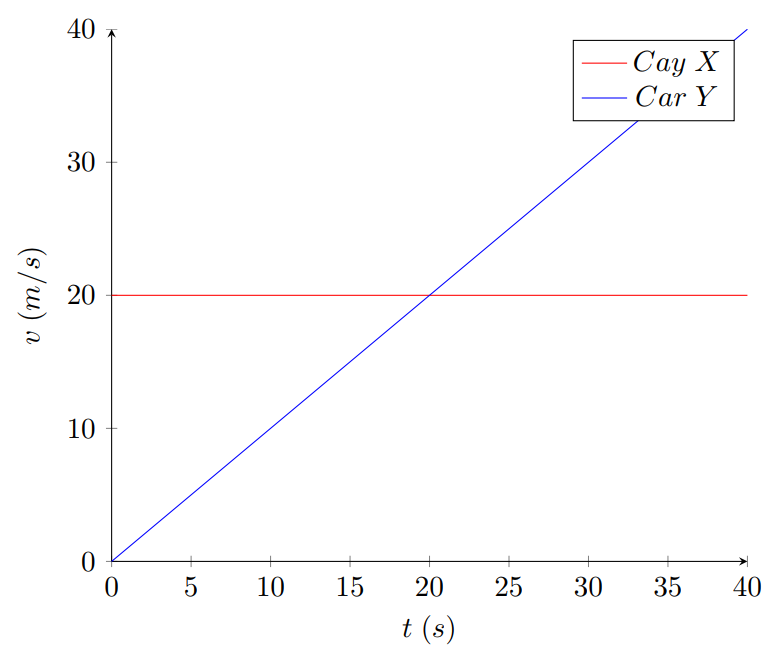
\includegraphics{Figures/Figure11}
\\
At time t=0, car X traveling with speed $v_0$ passes car Y, which is just starting to move. Both cars then travel on two parallel lanes of the same straight road. The graphs of speed $v$ versus time $t$ for both cars are shown above. Use this information for the next two questions.

%%%%%%%%%%%%%%%%%%%%%%%%%%%%%%%%%%
%%%%%%%%%%%%%%%%%%%%%%%%%%%%%%%%%%
%%%%%%%%%%%%%%%%%%%%%%%%%%%%%%%%%%

\begin{question}
(AP) Which of the following is true at time t=20 seconds?
\begin{enumerate}[label=(\alph*)]
    \item Car Y is behind car X
    \item Car Y is passing car X
    \item Car Y is in front of Car X
    \item Both Cars have the same acceleration
    \item Car X is accelerating faster than car Y
\end{enumerate}
\end{question}

\begin{solution}
A (hint: the area underneath v(t) is position)
\end{solution}

%%%%%%%%%%%%%%%%%%%%%%%%%%%%%%%%%%
%%%%%%%%%%%%%%%%%%%%%%%%%%%%%%%%%%
%%%%%%%%%%%%%%%%%%%%%%%%%%%%%%%%%%
\newpage
\begin{question}
(AP) From time $t=0$ to time $t=40\;seconds$, the areas under both curves are equal. Therefore, which of the following is true at time $t=40\;seconds$?
\begin{enumerate}[label=(\alph*)]
    \item Car Y is behind car X
    \item Car Y is passing car X
    \item Car Y is in front of Car X
    \item Both Cars have the same acceleration
    \item Car X is accelerating faster than car Y
\end{enumerate}
\end{question}

\begin{solution}
B (hint: equal areas mean currently, they're in the same position)
\end{solution}

%%%%%%%%%%%%%%%%%%%%%%%%%%%%%%%%%%
%%%%%%%%%%%%%%%%%%%%%%%%%%%%%%%%%%
%%%%%%%%%%%%%%%%%%%%%%%%%%%%%%%%%%

\begin{question}
(AP) A body moving in the positive x direction passes the origin at time $t=0$. Between $t=0$ and $t=1\;sec$, the body has a constant speed of $24\frac{m}{s}$. At $t=1\;sec$ the body is given a constant acceleration of 6 meters per second squared in the negative x direction. The positive x of the body at t=11 seconds is:
\begin{multicols}{5}
\begin{enumerate}[label=(\alph*)]
    \item +99 m
    \item +36 m
    \item -36 m
    \item -75 m
    \item -99 m
\end{enumerate}
\end{multicols}
\end{question}

\begin{solution}
C (Hint: use (1.3))
\end{solution}

%%%%%%%%%%%%%%%%%%%%%%%%%%%%%%%%%%
%%%%%%%%%%%%%%%%%%%%%%%%%%%%%%%%%%
%%%%%%%%%%%%%%%%%%%%%%%%%%%%%%%%%%

\begin{question}
(AP) An object released from rest at time t=0 slides down a frictionless incline a distance of 1 meter during the first second. The distance traveled by the object during the time itnerval from t=1 second to t=2 seconds is:
\begin{multicols}{5}
\begin{enumerate}[label=(\alph*)]
    \item 1 m
    \item 2 m
    \item 3 m
    \item 4 m
    \item 5 m
\end{enumerate}
\end{multicols}
\end{question}

\begin{solution}
C (Hint: The acceleration due to gravity isn't g!)
\end{solution}

%%%%%%%%%%%%%%%%%%%%%%%%%%%%%%%%%%
%%%%%%%%%%%%%%%%%%%%%%%%%%%%%%%%%%
%%%%%%%%%%%%%%%%%%%%%%%%%%%%%%%%%%

\begin{question}
(AP) Two people are in a boat that is capable of a maximum speed of 5 kilometers per hour in still water, and wish to cross a river 1 kilometer wide to a point directly across from their starting point. If the speed of the water in the river is 5 kilometers per hour, how much time is required for the crossing?
\begin{multicols}{5}
\begin{enumerate}[label=(\alph*)]
    \item 0.05 hr
    \item 0.1 hr
    \item 1 hr
    \item 10 hr
    \item \small{impossible}
\end{enumerate}
\end{multicols}
\end{question}

\begin{solution}
E (Hint: This is actually a stupid question. Use common sense!)
\end{solution}

%%%%%%%%%%%%%%%%%%%%%%%%%%%%%%%%%%
%%%%%%%%%%%%%%%%%%%%%%%%%%%%%%%%%%
%%%%%%%%%%%%%%%%%%%%%%%%%%%%%%%%%%

\begin{question}
(AP) A projectile is fired from the surface of the Earth with a speed of 200 meters per second at an angle of $30\deg$ above the horizontal. If the ground is level, what is the maximum height reached by the projectile?
\begin{multicols}{5}
\begin{enumerate}[label=(\alph*)]
    \item 5 m
    \item 10 m
    \item 500 m
    \item 1000 m
    \item 2000 m
\end{enumerate}
\end{multicols}
\end{question}

\begin{solution}
C (Hint: Velocity at the top of the trajectory is zero!)
\end{solution}

%%%%%%%%%%%%%%%%%%%%%%%%%%%%%%%%%%
%%%%%%%%%%%%%%%%%%%%%%%%%%%%%%%%%%
%%%%%%%%%%%%%%%%%%%%%%%%%%%%%%%%%%

\begin{question}
(AP) A rock is dropped from the top of a 45 meter tower, and at the same time a ball is thrown from the top of the tower in a horizontal direction. Air resistance is negligible. The ball and the rock hit the ground a distance of 30 meters apart. The horizontal velocity of the ball thrown was most nearly:
\begin{multicols}{5}
\begin{enumerate}[label=(\alph*)]
    \item 5 m/s
    \item 11 m/s
    \item 14.1 m/s
    \item 20 m/s
    \item 28.3 m/s
\end{enumerate}
\end{multicols}
\end{question}

\begin{solution}
B (Hint: First, you'll need to figure out the time it took, then solve for the speed)
\end{solution}

%%%%%%%%%%%%%%%%%%%%%%%%%%%%%%%%%%
%%%%%%%%%%%%%%%%%%%%%%%%%%%%%%%%%%
%%%%%%%%%%%%%%%%%%%%%%%%%%%%%%%%%%

\begin{question}
(AP) In the absense of air friction, an object dropped near the surface of the Earth experiences a constant acceleration of about $9.8\frac{m}{s^2}$. This means that the
\begin{enumerate}[label=(\alph*)]
    \item speed of the object increases 9.8 m/s during each second
    \item speed of the object as it falls is 9.8 m/s
    \item object falls 9.8 meters during each second
    \item object falls 9.8 meters during the first second only
\end{enumerate}

\end{question}

\begin{solution}
A (Hint: Go over what acceleration is again)
\end{solution}


%%%%%%%%%%%%%%%%%%%%%%%%%%%%%%%%%%
%%%%%%%%%%%%%%%%%%%%%%%%%%%%%%%%%%
%%%%%%%%%%%%%%%%%%%%%%%%%%%%%%%%%%

\begin{question}
(AP) A 500 kilogram sports car accelerates uniformly from rest, reaching a speed of 30 meters per second in 6 seconds. During the 6 seconds, the car has traveled a distance of:
\begin{multicols}{5}
\begin{enumerate}[label=(\alph*)]
    \item 15 m
    \item 30 m
    \item 60 m
    \item 90 m
    \item 180 m
\end{enumerate}
\end{multicols}
\end{question}

\begin{solution}
D (Hint: First solve for acceleration, then solve for distance)
\end{solution}


%%%%%%%%%%%%%%%%%%%%%%%%%%%%%%%%%%
%%%%%%%%%%%%%%%%%%%%%%%%%%%%%%%%%%
%%%%%%%%%%%%%%%%%%%%%%%%%%%%%%%%%%

\begin{question}
(AP) An object is shot vertically upward into the air with a positive velocity. Which of the following correctly describes the velocity and acceleration of the object at its maximum elevation?

\begin{tabular}{ |c|c|c| } 
\hline
       & Velocity & Acceleration \\ 
 A     & Positive & Positive \\ 
 B     & Zero & Zero \\ 
 C     & Negative & Negative \\ 
 D     & Zero & Negative \\ 
 E     & Positive & Negative \\
\end{tabular}

\end{question}

\begin{solution}
E (Hint: It's going up, but slowing down!)
\end{solution}

%%%%%%%%%%%%%%%%%%%%%%%%%%%%%%%%%%
%%%%%%%%%%%%%%%%%%%%%%%%%%%%%%%%%%
%%%%%%%%%%%%%%%%%%%%%%%%%%%%%%%%%%
\newpage
\begin{question}
(AP) A spring-loaded gun can fire a projectile to a height h if it is fired straight up. If the same gun is pointed at an angle of $45\deg$ from the vertical, what maximum height can now be reached by the projectile?
\begin{multicols}{5}
\begin{enumerate}[label=(\alph*)]
    \item $\frac{h}{4}$
    \item $\frac{h}{2\sqrt{2}}$
    \item $\frac{h}{2}$
    \item $\frac{h}{\sqrt{2}}$
    \item $h$
\end{enumerate}
\end{multicols}
\end{question}

\begin{solution}
D (Hint: It's very similar to 1.3.8)
\end{solution}

%%%%%%%%%%%%%%%%%%%%%%%%%%%%%%%%%%
%%%%%%%%%%%%%%%%%%%%%%%%%%%%%%%%%%
%%%%%%%%%%%%%%%%%%%%%%%%%%%%%%%%%%

\begin{question}
(AP) The velocity of a projectile at launch has a horizontal component $v_h$ and a vertical component $v_v$. Air resistance is negligible. When the projectile is at the highest point of its trajectory, which of the following show the vertical and horizontal components of its velocity and the vertical component of its acceleration?

\begin{tabular}{ |c|c|c|c| } 
 \hline
       & Vertical Velocity & Horizontal Velocity & Vertical Acceleration \\ 
 A     & $v_v$ & $v_h$ & 0\\  
 B     & $v_v$ & 0 & 0\\ 
 C     & 0 & $v_h$ & 0\\ 
 D     & 0 & 0 & g\\ 
 E     & 0 & $v_h$ & g\\ 
 \hline
\end{tabular}

\end{question}

\begin{solution}
E (Hint: It's still moving forward, but it's not moving up anymore. Something's pulling it down!)
\end{solution}

%%%%%%%%%%%%%%%%%%%%%%%%%%%%%%%%%%
%%%%%%%%%%%%%%%%%%%%%%%%%%%%%%%%%%
%%%%%%%%%%%%%%%%%%%%%%%%%%%%%%%%%%

\begin{question}
(AP) A target $T$ lies flat on the ground 3 m from the side of a building that  is 10 m tall. A student rolls a ball off the horizontal roof of the building in the direction of the target. Air Resistance is negligible. The horizontal speed with which the ball must leave the roof if it is to strike the target is most nearly:

\begin{multicols}{5}
\begin{enumerate}[label=(\alph*)]
    \item $\frac{3}{10}\frac{m}{s}$
    \item $\sqrt{2}\frac{m}{s}$
    \item $\frac{3}{\sqrt{2}}\frac{m}{s}$
    \item $3\frac{m}{s}$
    \item $10\sqrt{\frac{10}{3}}\frac{m}{s}$
\end{enumerate}
\end{multicols}

\end{question}

\begin{solution}
C (Hint: Solve for time, then solve for velocity)
\end{solution}

%%%%%%%%%%%%%%%%%%%%%%%%%%%%%%%%%%
%%%%%%%%%%%%%%%%%%%%%%%%%%%%%%%%%%
%%%%%%%%%%%%%%%%%%%%%%%%%%%%%%%%%%

\begin{question}
(AP) An object is dropped from rest from the top of a 400 m cliff on Earth. If air resistance is negligible, what is the distance the object travels during the first 6 s of its fall?

\begin{multicols}{5}
\begin{enumerate}[label=(\alph*)]
    \item 30 m
    \item 60 m
    \item 120 m
    \item 180 m
    \item 360 m
\end{enumerate}
\end{multicols}

\end{question}

\begin{solution}
D (Hint: For problems like this, double check by making sure the time it takes to fall 300 metres is over 6 seconds)
\end{solution}

%%%%%%%%%%%%%%%%%%%%%%%%%%%%%%%%%%
%%%%%%%%%%%%%%%%%%%%%%%%%%%%%%%%%%
%%%%%%%%%%%%%%%%%%%%%%%%%%%%%%%%%%
\newpage
\begin{question}
(AP) A student is testing the kinematic equations for uniformly accelerated motion by measuring the time it takes for light-weight plastic balls to fall to the floor from a height of 3 m in the lab. The student predicts the time to fall using g as 9.80 m/s2 but finds the measured time to be 35\% greater. Which of the following is the most likely cause of the large percent error?   

\begin{enumerate}[label=(\alph*)]
    \item The acceleration due to gravity is 70\% greater than $9.8\frac{m}{s^2}$
    \item The acceleration due to gravity is 70\% less than $9.8\frac{m}{s^2}$
    \item Air resistance increases the downward acceleration
    \item The acceleration of the plastic balls is not uniform
    \item The plastic balls are not truly spherical
\end{enumerate}

\end{question}

\begin{solution}
D (Hint: Use a process of elimination!)
\end{solution}

%%%%%%%%%%%%%%%%%%%%%%%%%%%%%%%%%%
%%%%%%%%%%%%%%%%%%%%%%%%%%%%%%%%%%
%%%%%%%%%%%%%%%%%%%%%%%%%%%%%%%%%%

\begin{question}
(AP) An object is thrown with velocity v from the edge of a cliff above level ground. Neglect air resistance. In order for the object to travel a maximum horizontal distance from the cliff before hitting the ground, the throw should be at an angle $\theta$ with respect to the horizontal of

\begin{enumerate}[label=(\alph*)]
    \item Greater than $60\deg$ above the horizontal
    \item greater than $45\deg$ but less than $60\deg$ above the horizontal
    \item greater than zero but less than $45\deg$ above the horizontal
    \item zero
    \item greater than zero but less than $45\deg$ below the horizontal
\end{enumerate}

\end{question}

\begin{solution}
C (Hint: If two trajectories ever cross paths, the one with the higher x velocity will land furthest)
\end{solution}

%%%%%%%%%%%%%%%%%%%%%%%%%%%%%%%%%%
%%%%%%%%%%%%%%%%%%%%%%%%%%%%%%%%%%
%%%%%%%%%%%%%%%%%%%%%%%%%%%%%%%%%%
\newpage
Starting from rest, a vehicle accelerates on a straight level road at the rate of $4 \frac{m}{s^2}$ for 5 seconds. Use this information for the next two questions:

%%%%%%%%%%%%%%%%%%%%%%%%%%%%%%%%%%
%%%%%%%%%%%%%%%%%%%%%%%%%%%%%%%%%%
%%%%%%%%%%%%%%%%%%%%%%%%%%%%%%%%%%

\begin{question}
(AP) What is the speed of the vehicle at the end of this time interval?

\begin{multicols}{5}
\begin{enumerate}[label=(\alph*)]
    \item 1.3 m/s
    \item 10 m/s
    \item 20 m/s
    \item 80 m/s
    \item 100 m/s
\end{enumerate}
\end{multicols}
\end{question}

\begin{solution}
C (Hint: Use 1.2)
\end{solution}

%%%%%%%%%%%%%%%%%%%%%%%%%%%%%%%%%%
%%%%%%%%%%%%%%%%%%%%%%%%%%%%%%%%%%
%%%%%%%%%%%%%%%%%%%%%%%%%%%%%%%%%%

\begin{question}
(AP) What is the total distance the vehicle travels during this time interval?
\begin{multicols}{5}
\begin{enumerate}[label=(\alph*)]
    \item 10 m
    \item 20 m
    \item 25 m
    \item 40 m
    \item 50 m
\end{enumerate}
\end{multicols}
\end{question}

\begin{solution}
E (Hint: Use 1.3)
\end{solution}

%%%%%%%%%%%%%%%%%%%%%%%%%%%%%%%%%%
%%%%%%%%%%%%%%%%%%%%%%%%%%%%%%%%%%
%%%%%%%%%%%%%%%%%%%%%%%%%%%%%%%%%%

\begin{question}
(AP) If air resistance is negligible, the speed of a 2 kg sphere that falls from rest through a vertical displacement of 0.2 m is most nearly
\begin{multicols}{5}
\begin{enumerate}[label=(\alph*)]
    \item 1 m/s
    \item 2 m/s
    \item 3 m/s
    \item 4 m/s
    \item 5 m/s
\end{enumerate}
\end{multicols}
\end{question}

\begin{solution}
E (Hint: Use 1.3)
\end{solution}

%%%%%%%%%%%%%%%%%%%%%%%%%%%%%%%%%%
%%%%%%%%%%%%%%%%%%%%%%%%%%%%%%%%%%
%%%%%%%%%%%%%%%%%%%%%%%%%%%%%%%%%%

\begin{question}
(AP) A projectile is launched from level ground with an initial speed $v_0$ at an angle $\theta$ with the horizontal. If air resistance is negligible, how long will the projectile remain in the air?
\begin{multicols}{5}
\begin{enumerate}[label=(\alph*)]
    \item $\frac{2v_0}{g}$
    \item $\frac{2v_0cos(\theta)}{g}$
    \item $\frac{v_0cos(\theta)}{g}$
    \item $\frac{v_0sin(\theta)}{g}$
    \item $\frac{2v_0sin(\theta)}{g}$
\end{enumerate}
\end{multicols}
\end{question}

\begin{solution}
E (Hint: The original and final speed is the same, due to the symmetry of the parabola)
\end{solution}

%%%%%%%%%%%%%%%%%%%%%%%%%%%%%%%%%%
%%%%%%%%%%%%%%%%%%%%%%%%%%%%%%%%%%
%%%%%%%%%%%%%%%%%%%%%%%%%%%%%%%%%%

\begin{question}
(AP) An object of unknown mass is initially at rest and dropped from a height h. It reaches the ground with a velocity $v_1$ The same object is then raised again to the same height h but this time is thrown downward with velocity $v_1$ It now reaches the ground with a new velocity $v_2$. How is $v_2$ related to $v_1$? 
\begin{multicols}{5}
\begin{enumerate}[label=(\alph*)]
    \item $v_2 = \frac{v_1}{2}$
    \item $v_2 = v_1$
    \item $v_2 = \frac{v_1}{\sqrt{2}}$
    \item $v_2 = 2v_1$
    \item $v_2 = 4v_1$
\end{enumerate}
\end{multicols}
\end{question}

\begin{solution}
E (Hint: Use 1.4 to solve solve for $v_1$ then use 1.4 again to solve for $v_2$ in terms of $v_1$. Then substitute.)
\end{solution}

%%%%%%%%%%%%%%%%%%%%%%%%%%%%%%%%%%
%%%%%%%%%%%%%%%%%%%%%%%%%%%%%%%%%%
%%%%%%%%%%%%%%%%%%%%%%%%%%%%%%%%%%
\newpage
\begin{question}
The velocity function for an object falling from rest under the influence of gravity and air resistance is shown below. Which of the following statements about x(t) are consistent with this velocity function?

% \begin{tikzpicture}

% \begin{axis}[
%     axis lines = left,
%     xlabel = $t\;(s)$,
%     ylabel = {$v\;(m/s)$},
% ]

% %Below the black is defined
% \addplot [
%     domain=5:100,
%     samples=100, 
%     color=black,
% ]
% {0.3};
% \addlegendentry{terminal velocity}
% %Below the red is defined
% \addplot [
%     domain=0:100,
%     range=0:2,
%     samples=100, 
%     color=red,
% ]
% {x/(10+3.333*x)};

% %Below the black is defined
% \addplot [
%     domain=1:100,
%     samples=100, 
%     color=white,
% ]
% {0.5};

% \end{axis}
% \end{tikzpicture}
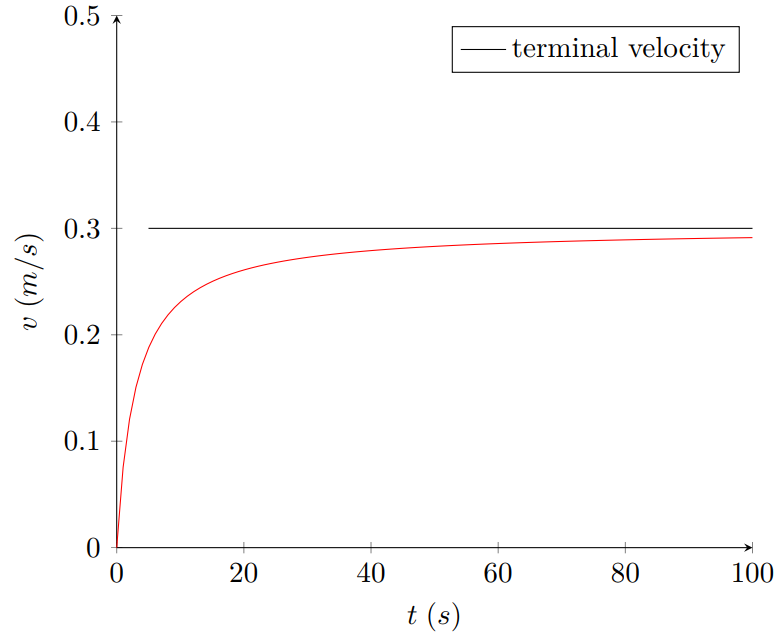
\includegraphics{Figures/Figure12}

\begin{tabular}{ |c|c|c|c| } 
 \hline
       & Y-Intercept & Starting Acceleration & Asymptote \\ 
 A     & Zero & Positive & Slant (Oblique)\\  
 B     & Positive & Positive & Horizontal\\ 
 C     & Zero & Negative & Slant (Oblique)\\ 
 D     & Negative & Negative & Horizontal\\ 
 E     & Zero & Positive & No\\ 
 \hline
\end{tabular}

\end{question}

\begin{solution}
A (Hint: Sketch it out!)
\end{solution}

%%%%%%%%%%%%%%%%%%%%%%%%%%%%%%%%%%
%%%%%%%%%%%%%%%%%%%%%%%%%%%%%%%%%%
%%%%%%%%%%%%%%%%%%%%%%%%%%%%%%%%%%

\begin{question}
A particle moves along the x-axis with a nonconstant acceleration described by $a=12t$, where a is in meters per second squared and t is in seconds. If the particle starts from rest so that its speed $v$ and position $x$ are zero when t=0, where is it located when $t=2\;sec$?
\begin{multicols}{5}
\begin{enumerate}
    \item 5 m
    \item 10 m
    \item 500 m
    \item 1000 m
    \item 2000 m
\end{enumerate}
\end{multicols}
\end{question}

\begin{solution}
B (Hint: take the integral two times!)
\end{solution}

%%%%%%%%%%%%%%%%%%%%%%%%%%%%%%%%%%
%%%%%%%%%%%%%%%%%%%%%%%%%%%%%%%%%%
%%%%%%%%%%%%%%%%%%%%%%%%%%%%%%%%%%
\newpage
\begin{question}
Vectors $v_1$ and $v_2$ shown below have equal magnitudes. The vectors represent the velocities of an object at times $t_1$, and $t_2$, respectively. The average acceleration of the object between time $t_1$ and $t_2$ was directed:

% \begin{tikzpicture}
%   \draw[thin,gray!40] (-2,-2) grid (2,2);
%   \draw[<->] (-2,0)--(2,0) node[right]{$E$};
%   \draw[<->] (0,-2)--(0,2) node[above]{$N$};
%   \draw[line width=2pt,blue,-stealth](0,0)--(1,0.5) node[anchor=south west]{$\boldsymbol{v_1}$};
%   \draw[line width=2pt,red,-stealth](0,0)--(0,1) node[anchor=north east]{$\boldsymbol{v_2}$};
% \end{tikzpicture}
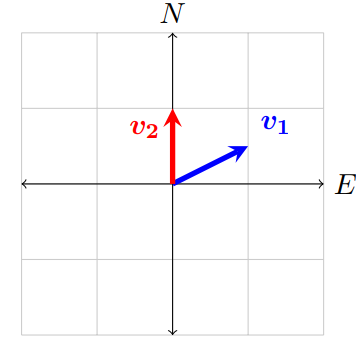
\includegraphics{Figures/Figure13}
\begin{multicols}{4}
\begin{enumerate}[label=(\alph*)]
    \item North
    \item West
    \item North of East
    \item North of West
\end{enumerate}
\end{multicols}

\end{question}

\begin{solution}
D (Hint: We're not looking at the location of $v$. We're looking at how $v$ changes.
\end{solution}

%%%%%%%%%%%%%%%%%%%%%%%%%%%%%%%%%%
%%%%%%%%%%%%%%%%%%%%%%%%%%%%%%%%%%
%%%%%%%%%%%%%%%%%%%%%%%%%%%%%%%%%%

\begin{question}
An object is thrown vertically upward in a region where g is constant and air resistance is negligible. Its speed is recorded from the moment it leaves the thrower's hand until it reaches its maximum height. Which of the following graphs best represent the object's speed $v$ versus time $t$ \footnote{If you can't distinguish between the colors, A, B, C, D are labelled in order of the end behaviour of each line}

% \begin{tikzpicture}
% \begin{axis}[
%     axis lines = left,
%     xlabel = $t$,
%     ylabel = {$v$},
% ]

% %A
% \addplot [
%     domain=0:1,
%     samples=100, 
%     color=blue,
% ]
% {e^x-1};
% \addlegendentry{A}

% %B
% \addplot [
%     domain=0:1,
%     samples=100, 
%     color=red,
% ]
% {x};
% \addlegendentry{B}

% %C
% \addplot [
%     domain=0:1,
%     samples=100, 
%     color=black,
% ]
% {ln(x+1)};
% \addlegendentry{C}

% %D
% \addplot [
%     domain=0:1,
%     samples=100, 
%     color=green,
% ]
% {1-x};
% \addlegendentry{D}

% \end{axis}
% \end{tikzpicture}

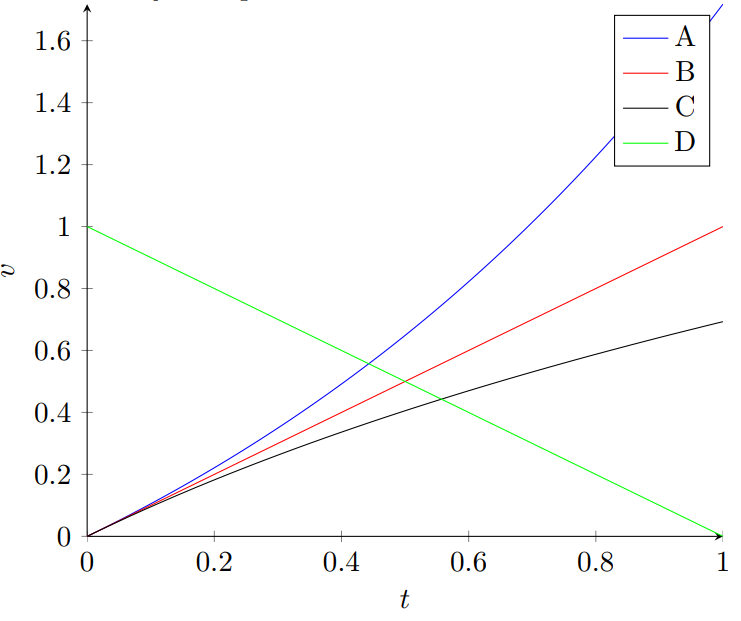
\includegraphics{Figures/Figure14}

\end{question}
\newpage
An object moving in a straight line has a velocity v in meters per second that varies with time t in seconds according to the following function: $v=4+0.5t^2$. Use this information to answer the next two questions:

%%%%%%%%%%%%%%%%%%%%%%%%%%%%%%%%%%
%%%%%%%%%%%%%%%%%%%%%%%%%%%%%%%%%%
%%%%%%%%%%%%%%%%%%%%%%%%%%%%%%%%%%

\begin{question}
The instantaneous acceleration of the object at t = 2 seconds is:
\begin{multicols}{5}
\begin{enumerate}
    \item $2\frac{m}{s^2}$
    \item $4\frac{m}{s^2}$
    \item $5\frac{m}{s^2}$
    \item $6\frac{m}{s^2}$
    \item $8\frac{m}{s^2}$
\end{enumerate}
\end{multicols}
\end{question}

\begin{solution}
A (Acceleration is the first derivative of velocity)
\end{solution}

%%%%%%%%%%%%%%%%%%%%%%%%%%%%%%%%%%
%%%%%%%%%%%%%%%%%%%%%%%%%%%%%%%%%%
%%%%%%%%%%%%%%%%%%%%%%%%%%%%%%%%%%

\begin{question}
The displacement of the object between t=0 and t=6 seconds is:
\begin{multicols}{5}
\begin{enumerate}
    \item 22 m
    \item 28 m
    \item 40 m
    \item 42 m
    \item 60 m
\end{enumerate}
\end{multicols}
\end{question}

\begin{solution}
E (Take the definite integral with 0 and 6 as bounds!)
\end{solution}

%%%%%%%%%%%%%%%%%%%%%%%%%%%%%%%%%%
%%%%%%%%%%%%%%%%%%%%%%%%%%%%%%%%%%
%%%%%%%%%%%%%%%%%%%%%%%%%%%%%%%%%%

\begin{question}
The position of an object is given by the equation $x=3t^2+1.5t+4.5$ where x is in meters and t is in seconds. What is the instantaneous acceleration of the object at $t=3\;sec$?

\begin{multicols}{5}
\begin{enumerate}
    \item $3 \frac{m}{s^2}$
    \item $6 \frac{m}{s^2}$
    \item $9 \frac{m}{s^2}$
    \item $19.5 \frac{m}{s^2}$
    \item $36 \frac{m}{s^2}$
\end{enumerate}
\end{multicols}
\end{question}

\begin{solution}
B (Hint: Acceleration is the second derivative of position)
\end{solution}

%%%%%%%%%%%%%%%%%%%%%%%%%%%%%%%%%%
%%%%%%%%%%%%%%%%%%%%%%%%%%%%%%%%%%
%%%%%%%%%%%%%%%%%%%%%%%%%%%%%%%%%%

\begin{question}
At a particular instant, a stationary observer on the ground sees a package falling with a speed of $v_1$ at an angle to the vertical. To a pilot flying horizontaly at constant speed relative to the ground, the package appears to be falling vertically with a speed $v_2$ at that instant. What is the speed of the pilot relative to the ground?

\begin{multicols}{5}
\begin{enumerate}
    \item $v_1+v_2$
    \item $v_1-v_2$
    \item $v_2-v_1$
    \item $\sqrt{v_1^2-v_2^2}$
    \item $\sqrt{v_1^2+v_2^2}$
\end{enumerate}
\end{multicols}
\end{question}

\begin{solution}
D (Hint: Pythagorean Theorem!)
\end{solution}

%%%%%%%%%%%%%%%%%%%%%%%%%%%%%%%%%%
%%%%%%%%%%%%%%%%%%%%%%%%%%%%%%%%%%
%%%%%%%%%%%%%%%%%%%%%%%%%%%%%%%%%%
%%%%%%%%%%%%%%%%%%%%%%%%%%%%%%%%%%
%%%%%%%%%%%%%%%%%%%%%%%%%%%%%%%%%%
%%%%%%%%%%%%%%%%%%%%%%%%%%%%%%%%%%
%%%%%%%%%%%%%%%%%%%%%%%%%%%%%%%%%%
%%%%%%%%%%%%%%%%%%%%%%%%%%%%%%%%%%
%%%%%%%%%%%%%%%%%%%%%%%%%%%%%%%%%%
%%%%%%%%%%%%%%%%%%%%%%%%%%%%%%%%%%
%%%%%%%%%%%%%%%%%%%%%%%%%%%%%%%%%%
%%%%%%%%%%%%%%%%%%%%%%%%%%%%%%%%%%
%%%%%%%%%%%%%%%%%%%%%%%%%%%%%%%%%%
%%%%%%%%%%%%%%%%%%%%%%%%%%%%%%%%%%
%%%%%%%%%%%%%%%%%%%%%%%%%%%%%%%%%%

\newpage
\section{Solutions}
\printsolutions

%%%%%%%%%%%%%%%%
% Electrostatics  %
%%%%%%%%%%%%%%%%
\chapter{Coulomb's Law (Point Particle)}
You are beginning your studies of electrostatics, the study of stationary charges. This chapter will only focus on coulomb's law and the applications on single particles. If you think this is hard, you'll love the next chapters :)
\\\\
There are many similarities between electrostatics and gravitation. In this chapter, we will be focusing more on Coulomb's law and hopefully point out many parallels between two seemingly unrelated fields (pun intended)


\section{Equations}
\begin{equation}
    F=\frac{|Q_1Q_2|}{4\pi\epsilon_0R^2}
\end{equation}
\begin{equation}
    \frac{F}{Q}=\frac{F_{any\;charge}}{Q_{any\;charge}}=E
\end{equation}
\begin{equation}
    E_{net}=E_1+E_2+E_3+\dots+E_N
\end{equation}
\begin{equation}
    V=\frac{U}{Q} \iff
    \Delta V=\frac{\Delta U}{Q}
\end{equation}

Many textbooks will make the substitution for coulomb's constant: $k=\frac{1}{4\pi\epsilon_0}$ to simplify Coulomb's Law (2.1) However, it is generally preferred to keep it in the long form as the $\pi$ may cancel out with other terms.

\subsection*{Calculus}

The only calculus equation needed is a direct restatement of (2.4). Although it has an extremely trivial derivation for any calculus student, it is vital in solving many problems involving calculus.

\begin{equation}
    E_x=-\frac{dV}{dx}
\end{equation}

\section{Tricks}
\hfuzz=100pt 

\subsection{General Strategy}
The majority of problems in this chapter is focused on using Coulomb's Law. Because force is a vector, it can sometimes be hard to keep track of all the different directions. First, calculate the magnitude of each individual force, then break the force into components. Then, superimpose all the forces by summing them up.\footnote{Remember, you can't sum magnitudes, but you can sum vectors} If it is needed, convert back to magnitude only at the end.

\subsection{Analog to Gravitation}
Hopefully, you can already see the similarities between electrostatics and gravitation. If not, we will point it out below. The force between two charges is almost exactly equivalent to the force between two masses.

Coulomb's Law: $F=\frac{1}{4\pi\epsilon_0}\frac{Q_1Q_2}{R^2}$

Newton's Law of Gravitation: $F=G\frac{M_1M_2}{R^2}$

Notice how the gravitational constant is a direct analog to coulomb's constant and how mass is a direct analog to charge. Even the principle of superposition holds true for both gravitation and electrostatics. Furthermore, the electric field $E$ can also be seen as a direct analog to gravitational acceleration $g=G\frac{M}{R^2}$

\emph{Unlike} gravitation however, the force does not always act towards one direction. Masses can only attract one another, but charges can attract as well as repel. When two charges repel, their force is positive.

More similarities will be pointed out in the chapters to come.

\subsection{Electric Field Lines}
The electric field is a vector field, meaning it assigns a vector (basically an arrow) to every point in space, such as in the figure below. The red lines represent the electric field at that point and flow from positive charges to negative charges: \footnote{The contour lines are equipotential lines, discussed in the next section about Energy Conservation.}

\begin{center}
% \begin{tikzpicture}
% \begin{axis}[axis equal image,domain=-4.05:4.05,,xmin=-4,xmax=4,ymin=-4,ymax=4,samples=40,view={0}{90}]

%   \addplot3[contour gnuplot={number=50,labels=false, draw color=blue},thick,]
%               {abs(((1)/sqrt((x-2)^2+y^2) - (1)/sqrt((x+2)^2+y^2)))<4 ? ((1)/sqrt((x-2)^2+y^2) - (1)/sqrt((x+2)^2+y^2)) : NaN };
% %set to 18
%   \addplot3[contour gnuplot={number=18,labels=false, draw color=red},
%              thick,
%             ]
%              {abs(((x-2)/sqrt((x-2)^2+y^2) - (x+2)/sqrt((x+2)^2+y^2)))<10 ? ((x-2)/sqrt((x-2)^2+y^2) - (x+2)/sqrt((x+2)^2+y^2)) : NaN };
% \end{axis}
% \end{tikzpicture}
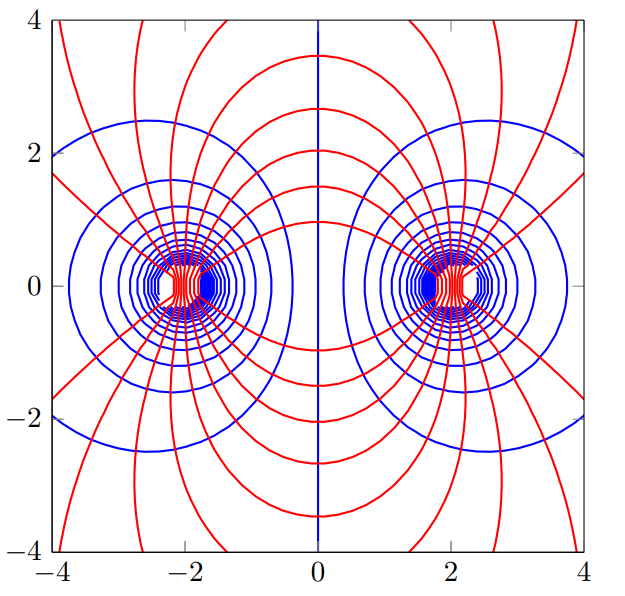
\includegraphics{Figures/Figure21}
\end{center}

Important properties of electric field lines which can be used in problem solving are listed below:
\begin{enumerate}
    \item The lines begin and end only on charges. As a result, the lines are spaced such that they are bunched more closely together in areas of strong field and spaced more widely apart in areas of weak field.
    \item Because the electric field can have only one unique direction at any location in space, the lines may never intersect in a location where the direction of the electric field is well defined
    \item The lines represent the direction of the force. In general, the lines do not represent the \emph{trajectory} of a particle moving only under the influence of the electric field.\footnote{Why? From mechanics, we know that for a particle to move along a curved path, it must have a radial acceleration. If a particle were moving along a curved electric field line, because the force is parallel to the field line, there would be no force providing the radial acceleration - that would be impossible!}
\end{enumerate}

\newpage
\subsection{Energy Conservation Problems}
Because potential, or voltage: $V$ is a measure of potential energy \emph{per} charge, it is easily used to calclate the potential energy of a specified charge and thus is useful in problems involving energy conservation.

Potential is a \emph{scaler} meaning we can assign a single value to every single point on the x,y plane. Because of this, we can represent potential in two dimensions using \emph{equipotential lines}, which are lines of constant potential in the two-dimensional plane. By providing a series of equipotential lines at equally spaced intervals (i.e., plotting when potential is 1V, 2V, 3V, and so on) a contour plot can be created similar to topographical maps that display different altitudes in different colors. Here are important properties of potential lines when problem solving
\begin{enumerate}
    \item Because potential is constant along an equipotential line, no force or work is required to move a charge along a given equipotentia line
    \item Recall $W=Fdcos(\theta)$ Because no work is required, this means $\theta$ must be $90^\circ$ meaning \emph{the equipotential lines is perpendicular to the electric field}
    \item When the electric field is stronger, the potential lines are bunched closer together. If you know calculus, you can use (2.5) to prove this.
\end{enumerate}

% \begin{tikzpicture}
% \begin{axis}[
%     view={0}{90},
%     clip = false,
%     xmin = -4,
%     xmax = 4,
%     ymin = -2.3,
%     ymax = 2.3,
%     point meta min = -4,
%     point meta max = 3,
%     y axis line style={draw opacity=0},
%     x axis line style={draw opacity=0},
%     xtick=\empty,
%     ytick=\empty,
%     unit vector ratio=1 1 1,
%     width=\linewidth,
%     colormap name=viridis
%     ]
% \addplot+[
%     no markers,
%     raw gnuplot,
%     contour prepared,
%     contour/labels=false
%     ] gnuplot {set samples 50, 50;
%             set isosamples 55, 55;
%             set contour base;
%             set cntrparam levels incremental -4,0.22,4;
%             set style data lines;
%             splot [-4:4] [-2.3:2.3] (-2/sqrt((x+2)**2+y**2)-1/sqrt((x-2)**2+y**2));
%             };
% \end{axis}
% \end{tikzpicture}
\begin{center}
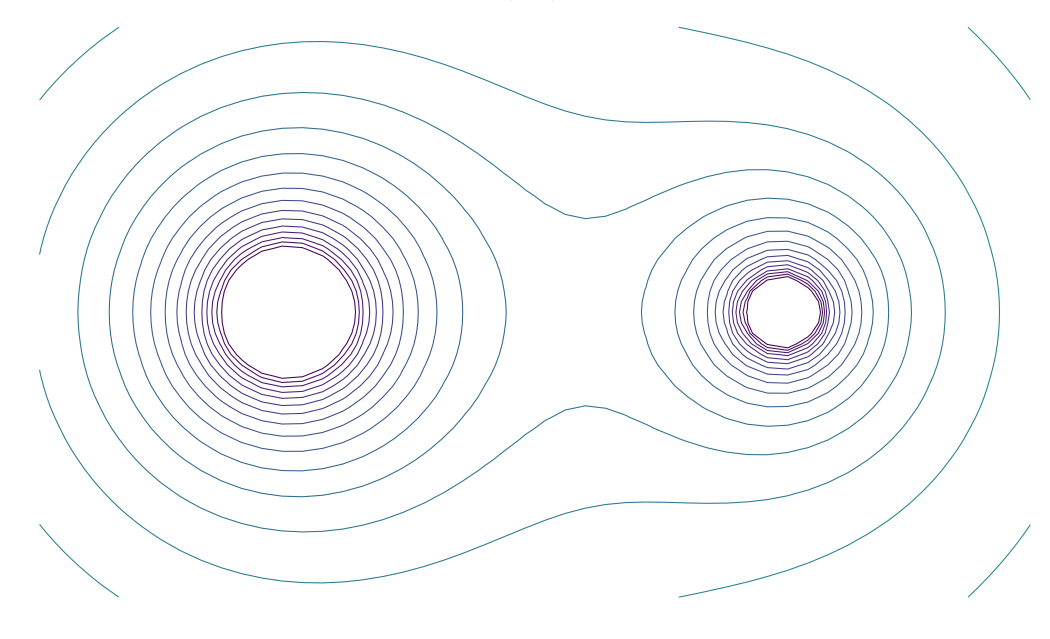
\includegraphics[scale=0.7]{Figures/Figure22}
\end{center}

Here is a sample contour plot of equipotential lines. Based solely on this diagram and using the tricks provided, can you:
\begin{enumerate}
    \item Identify the source of the charges?
    \item Identify where the electric field is weakest?
    \item Draw the electric field lines?
\end{enumerate}

\newpage
\section{Problems}
\SetupExSheets{
  question/post-body-hook = {%
    \hyperlink{sol:\CurrentQuestionID}{ (View Solution)}
  },
  solution/pre-hook = {
    \hypertarget{sol:\CurrentQuestionID}{}%
  } ,
  solution/pre-body-hook = {%
    \hyperref[qu:\CurrentQuestionID]{ (View Question)}\par
  }
}

\SetupExSheets{
  counter-format = ch.3.qu,
  headings=runin
} 

\subsection*{Regular}
%%%%%%%%%%%%%%%%%%%%%%%%%%%%%%%%%%
%%%%%%%%%%%%%%%%%%%%%%%%%%%%%%%%%%
%%%%%%%%%%%%%%%%%%%%%%%%%%%%%%%%%%

\begin{question}
What are the units for permittivity of free space $\epsilon_0$?

\end{question}

\begin{solution}

Rearrange the equation to solve for $\epsilon_0$, and give all variables a value of 1 in order to figure out the units for $\epsilon_0$. Please note, that we are giving everything a value of 1 for the sole purpose of making adding, multiplying, and dividing units much easier. It of course is not necessary, but helps to build an intuition of dimensional analysis.

The final value of course, is going to be incorrect, but we only care about the units. Because of this, we can ignore $2\pi$ since it is dimensionless.

\begin{equation*}
F = \frac{Q_1Q_2}{\epsilon_0R^2} \rightarrow
\epsilon_0 = \frac{Q_1Q_2}{FR^2} \rightarrow
\epsilon_0 = \frac{(1C)(1C)}{(1N)(1m)^2} \rightarrow
\epsilon_0 = (1C^2)(1N^{-1})(1m^{-2})
\end{equation*}

Thus $\epsilon_0$ has SI units of $C^2N^{-1}m^{-2}$
\end{solution}

%%%%%%%%%%%%%%%%%%%%%%%%%%%%%%%%%%
%%%%%%%%%%%%%%%%%%%%%%%%%%%%%%%%%%
%%%%%%%%%%%%%%%%%%%%%%%%%%%%%%%%%%

\begin{question}
Two $1\mu C$ charges lie at (1,0) and at (0,1).
\begin{enumerate}[label=(\alph*)]
    \item Calculate the magnitude of the force that $1-\mu C$ charge at (0,1) exerts on the $1\mu C$ charge at (1,0)
    \item Calculate the components of this force in the x- and y-directions and express the force as a vector.
\end{enumerate}
\end{question}

\begin{solution}

The first thing we do is draw a diagram: see the figure below. We are attempting to calculate the force, and since the charges of both particles are already given to us, we need to figure out the distance separating them which can be done using geometry.

\begin{center}
% \begin{tikzpicture}
% \begin{axis}[
%     axis lines=middle,
%     xmin=0, xmax=2,
%     ymin=0, ymax=2,
%     xtick=1, ytick=1,
%     xlabel = $x$,
%     ylabel = $y$,
% ]
% \addplot [only marks] table {
% 1   0
% 0   1
% };

% \addplot [domain=-10:10, samples=2, dashed] {1-x};
% \end{axis}
% \end{tikzpicture}
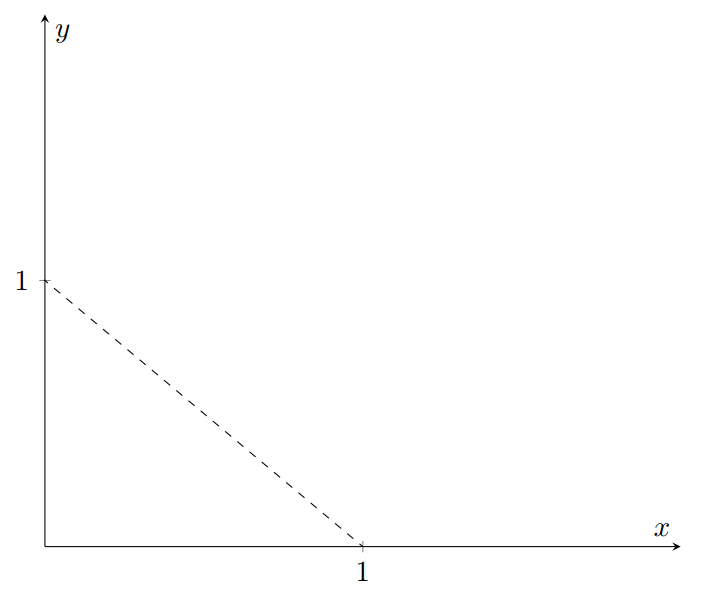
\includegraphics[scale=0.9]{Figures/Figure26}
\end{center}
(A) Thus the force is, using (2.1):
\begin{equation*}
    F=\frac{Q_1Q_2}{2\pi\epsilon_0R^2}=
    \frac{(1 \times 10^{-6}C)^2}
    {(2\pi)(8.854 \times 10^{-12}C^2N^{-1}m^{-2})(\sqrt{1^2 + 1^2}^2)}
\end{equation*}
\begin{equation*}
    F = 4.5 \times 10^{-3} N
\end{equation*}

(B) To calculate the components, we break up the \emph{magnitude} of the force we calculated in part A into components using standard geometry. Note that the y component is negative, because the charge at (1,0) will be wanting to move in the negative y and positive x direction.
\begin{equation*}
    \left\{
        \begin{array}{ll}
            F_x = (4.5 \times 10^{-3} N)cos(45^\circ) = 3.18 \times 10^{-3} N
            \\
            F_y = -(4.5 \times 10^{-3} N)cos(45^\circ) = -3.18 \times 10^{-3} N
        \end{array}
              \right.
\end{equation*}

Combining everything together gives the force vector:

\begin{equation*}
    \vec{F} = (3.18 \times 10^{-3} N)\hat{i} - 
              (3.18 \times 10^{-3} N)\hat{j}    
\end{equation*}

\end{solution}

%%%%%%%%%%%%%%%%%%%%%%%%%%%%%%%%%%
%%%%%%%%%%%%%%%%%%%%%%%%%%%%%%%%%%
%%%%%%%%%%%%%%%%%%%%%%%%%%%%%%%%%%

\begin{question}
A point charge +Q is located at the origin and a point charge -2Q is located at (1,0). Where is the electric field equal to zero? (Everything is in SI units)

\end{question}

\begin{solution}
The first thing to realize is that the only place the electric field can ever be zero is along the x-axis.\footnote{think about suspending an object under two magnets. It only works if it's directly underneath both of them!} Before we brute force, let's make a diagram and think about the question qualitatively.

% \begin{center}
%   \begin{tikzpicture}[scale=2]
%     \draw (-3,0) -- (3,0);
%     \foreach \i in {-3,-2,...,3} % numbers on line
%       \draw (\i,0.1) -- + (0,-0.2) node[below] {$\i$};
%     \fill[blue] (0,0) circle (0.5 mm);
%     \fill[red]  (1,0) circle (1 mm);
%   \end{tikzpicture}   
% \end{center}
\begin{center}
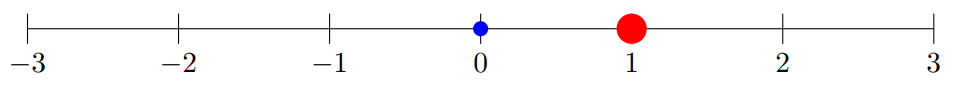
\includegraphics{Figures/Figure27}
\end{center}
Where on the x-axis should we look for solutions? We have three options:
\begin{enumerate}
    \item Between (0,0) and (1,0): both charges produce an electric field in the +x direction.
    \item Between (1,0) and $\infty$: In this region, the -2Q charge is always dominant, also providing a nonzero electric field.
    \item Between (0,0) and -$\infty$: In this region, when we are very close to the +Q charge, the +Q charge will dominate. However, as we move further and further away, the effects of distance will be less and less prominent and the -2Q charge will come to dominate. We will call this location (x,0)
\end{enumerate}
 
To do the math, we simply need to use superposition:

\begin{equation}
    E_{net} = E_{+Q} + E_{-2Q} \rightarrow
    0 = \frac{Q}{4\pi\epsilon_0x^2} + 
        \frac{-2Q}{4\pi\epsilon_0(1-x)^2}
\end{equation}
\begin{equation}
    \frac{Q}{4\pi\epsilon_0x^2} = 
    \frac{2Q}{4\pi\epsilon_0(1-x)^2} \rightarrow
    \frac{1}{x^2} = \frac{2}{(1-x)^2} \rightarrow
    2x^2 = (x+1)^2
\end{equation}

Solving this quadratic relation gives $x=-1\pm\sqrt{2}$. Since we already established that x is negative, we know the electric field is zero at $x=-1-\sqrt{2}$

\end{solution}

%%%%%%%%%%%%%%%%%%%%%%%%%%%%%%%%%%
%%%%%%%%%%%%%%%%%%%%%%%%%%%%%%%%%%
%%%%%%%%%%%%%%%%%%%%%%%%%%%%%%%%%%

\begin{question}
A point charge $Q_1$ is located at the origin and a point charge $Q_2$ is located at (5,0). Which of the following situations have a point or points where the potential is zero? (more than one may apply)

\begin{center}
\begin{tabular}{ |c|c|c| } 
 \hline
       & $Q_1$ & $Q_2$ \\ 
 I      & +q  & +3q  \\ 
 II     & -q  & +17q \\ 
 III    & -3q & -q   \\ 
 \hline
\end{tabular}
\end{center}

\end{question}


\begin{solution}
Using the superposition formula for potential, we see that it is only possible for potential to be zero, when the charges have opposite signs:

\begin{equation*}
    V_{net}=0=\frac{Q_1}{x^2}+\frac{Q_2}{(5-x)^2}
\end{equation*}

Therefore, II is the correct answer.

Another solution is to draw the graphs of V(x) for each individual charge, and then superposition them like in the following figure:

\begin{center}
% \begin{tikzpicture}
% \begin{axis}[
%     axis lines=middle,
%     xmin=-20, xmax=20,
%     ymin=-20, ymax=20,
%     xlabel = $x$,
%     ylabel = $V$,
% ]
% %Below the red is defined
% \addplot [
%     domain=-20:20, 
%     samples=100, 
%     color=red,
%     style={ultra thick}
% ]
% {-1/(x^2)};
% \addlegendentry{$V_{-q}$}

% %Here the blue is defined
% \addplot [
%     domain=-20:20, 
%     samples=100, 
%     color=blue,
%     style={ultra thick},
% ]
% {17*x/((6-x)^2)};
% \addlegendentry{$V_{17q}$}

% \end{axis}
% \end{tikzpicture}
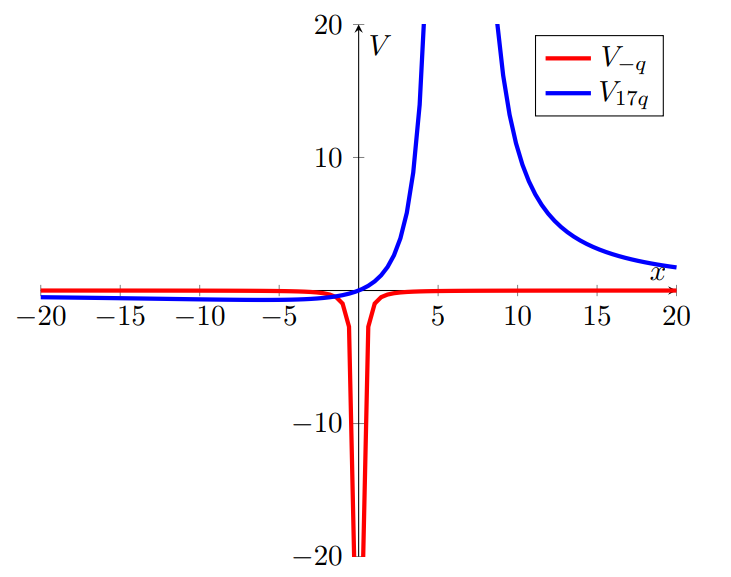
\includegraphics{Figures/Figure28}
\end{center}

All we need to prove is that if we add these two functions, it will have at least one real root. This proof will be left as an exercise to the reader.\footnote{Hint: You can prove this in two ways. Either use the mean value theorem, or notice that the peaks and troughs are located at different locations...}

\end{solution}

%%%%%%%%%%%%%%%%%%%%%%%%%%%%%%%%%%
%%%%%%%%%%%%%%%%%%%%%%%%%%%%%%%%%%
%%%%%%%%%%%%%%%%%%%%%%%%%%%%%%%%%%

\begin{question}
Which of the three charge distributions introduced in the previous exercise has point(s) where the electric field is zero?
\end{question}

\begin{solution}
We have already proved in an earlier exercise that in, the electric field between two opposite charges different in magnitude, there is one point where it is zero. In a charge distribution where both charges have equal signs, there is also one place where the electric field is zero, this time in between both charges. This is the spot where the charges cancel out.

The answer is I,II and III
\end{solution}

%%%%%%%%%%%%%%%%%%%%%%%%%%%%%%%%%%
%%%%%%%%%%%%%%%%%%%%%%%%%%%%%%%%%%
%%%%%%%%%%%%%%%%%%%%%%%%%%%%%%%%%%

\begin{question}
Points $Q_1$, $Q_2$, $Q_3$, and $Q_4$ are located at (-1,1),(1,1),(1,-1),(-1,-1) respectively. Which of the following charge distributions is the electric field zero at the origin?

\begin{center}
\begin{tabular}{ |c|c|c|c|c| } 
 \hline
       & $Q_1$ & $Q_2$ & $Q_3$ & $Q_4$ \\ 
 I        & +q  & +q & -q & -q  \\ 
 II       & +q  & -q & +q & -q  \\ 
 III      & +q  & -q & +q & +q  \\ 
 IV       & +q  & +q & +q & +q  \\ 
 V        & -q  & -q & -q & -q  \\ 
 \hline
\end{tabular}
\end{center}

\end{question}

\clearpage
\begin{solution}
The table is too confusing, so let's graph out $Q_1$, $Q_2$, $Q_3$, and $Q_4$ on a square:

\begin{center}
% \begin{tikzpicture}
% \draw (0,0) -- (0,2) -- (2,2) -- (2,0) -- (0,0);
% \node[above right] at (0,0) {$Q_4$};
% \node[below right] at (0,2) {$Q_1$};
% \node[below left] at (2,2) {$Q_2$};
% \node[above left] at (2,0) {$Q_3$};
% \end{tikzpicture}
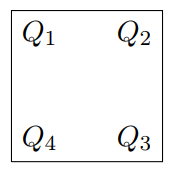
\includegraphics{Figures/Figure29}
\end{center}

In order for the center of the square to have a zero electric field, the electric field must be zero when the point charges are superimposed. We can superimpose the charges diagonally. This is possible if and only if $Q_1 = Q_3$ and $Q_2 = Q_4$ only II,IV,V satisfy this criteria.

\end{solution}

%%%%%%%%%%%%%%%%%%%%%%%%%%%%%%%%%%
%%%%%%%%%%%%%%%%%%%%%%%%%%%%%%%%%%
%%%%%%%%%%%%%%%%%%%%%%%%%%%%%%%%%%

\begin{question}
Which of the charge distributions introduced in the previous question is the potential zero at the origin?
\end{question}

\begin{solution}
The potential is zero at the origin if and only if the superposition of potential is equal to zero. Since potential is a scaler and all the charges are equidistant from the origin, this means that the total net charge at the origin has to be zero. In other words, the potential is zero, if and only if:

\begin{equation*}
    Q_1+Q_2+Q_3+Q_4=0
\end{equation*}

Only I, and II satisfy this criteria.

\end{solution}

%%%%%%%%%%%%%%%%%%%%%%%%%%%%%%%%%%
%%%%%%%%%%%%%%%%%%%%%%%%%%%%%%%%%%
%%%%%%%%%%%%%%%%%%%%%%%%%%%%%%%%%%

\begin{question}
Two positive charges +Q are located on the -axis at (0,a) and (0,-a), and a third charge -q is on the positive x-axis at (x,0). Find the electric field along the x-axis as a function of position E(x), due to the positive charges.
\end{question}

\begin{solution}
First, calculate the magnitude of the electric field as a function of position. Use the electric field equation (directly derived from Coulomb's Law) to figure out the electric field from one charge:

\begin{equation*}
    |E(x)| = \frac{Q}{4\pi\epsilon_0\sqrt{(x^2+a^2)}^2} =
             \frac{Q}{4\pi\epsilon_0(x^2+a^2)}
\end{equation*}

Now, to separate the magnitude of the electric field along the x-axis, using standard trigonometry techniques:

\begin{equation*}
    E(x)_x = |E(x)|cos(\theta) = |E(x)|(\frac{x}{\sqrt{(x^2+a^2)}})
    =
    \frac{Q}{4\pi\epsilon_0(x^2+a^2)}(\frac{x}{\sqrt{(x^2+a^2)}})
\end{equation*}

\begin{equation*}
    E(x)_x =
    \frac{Qx}{4\pi\epsilon_0(x^2+a^2)^{3/2}}
\end{equation*}

However, since we have two equally charged particles on the y-axis, we can superimpose them to get the final answer.\footnote{Because of symmetry, we can just multiply by two, instead of doing everything all over again}

\begin{equation*}
    E(x)_x =
    \frac{2Qx}{4\pi\epsilon_0(x^2+a^2)^{3/2}} =
    \frac{Qx}{2\pi\epsilon_0(x^2+a^2)^{3/2}}
\end{equation*}

\end{solution}

%%%%%%%%%%%%%%%%%%%%%%%%%%%%%%%%%%
%%%%%%%%%%%%%%%%%%%%%%%%%%%%%%%%%%
%%%%%%%%%%%%%%%%%%%%%%%%%%%%%%%%%%

\begin{question}
Two point charges +Q are located on the x-axis at (-d,0) and (d,0). Sketch the electric field $E(x)$ along the x-axis as a function of position.
\end{question}

\begin{solution}
First, graph the individual electric fields each charge produces, then sum it up. Please note we are NOT graphing $\frac{Q}{r\pi\epsilon_0x^2}$. That gives the magnitude of the electric field. Since electric field is a vector, anything that is to the left (negative x direction) of the charge will have a negative electric field.

The individual electric fields will look like:\footnote{Because of program graphing issues, the vertical asymptotes are shown, but in reality both ends should extend to $\pm \infty$ meaning these vertical lines are not \emph{real}}

\begin{center}
% \begin{tikzpicture}
% \begin{axis}[
%     axis lines=middle,
%     xmin=-10, xmax=10,
%     ymin=-10, ymax=10,
%     xlabel = $x$,
%     ylabel = $E$,
% ]
% %Below the red is defined
% \addplot [
%     domain=-10:10, 
%     samples=100, 
%     color=red,
%     style={ultra thick}
% ]
% {1/(x-3)};
% \addlegendentry{$E(x)_{Q1}$}

% %Here the blue is defined
% \addplot [
%     domain=-10:10, 
%     samples=100, 
%     color=blue,
%     style={ultra thick},
% ]
% {1/(x+3)};
% \addlegendentry{$E(x)_{Q2}$}

% \end{axis}
% \end{tikzpicture}
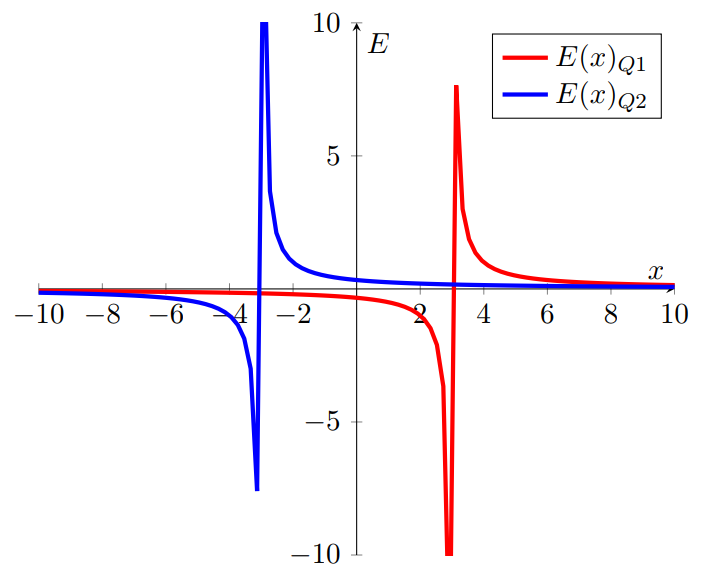
\includegraphics{Figures/Figure210}
\end{center}

And after they are superimposed, and added, it will look like:

\begin{center}
% \begin{tikzpicture}
% \begin{axis}[
%     axis lines=middle,
%     xmin=-10, xmax=10,
%     ymin=-10, ymax=10,
%     xlabel = $x$,
%     ylabel = $E$,
% ]

% %Here the purple is defined
% \addplot [
%     domain=-10:10, 
%     samples=100, 
%     color=purple,
%     style={ultra thick},
% ]
% {(1/(x+3))+(1/(x-3))};

% \end{axis}
% \end{tikzpicture}
% 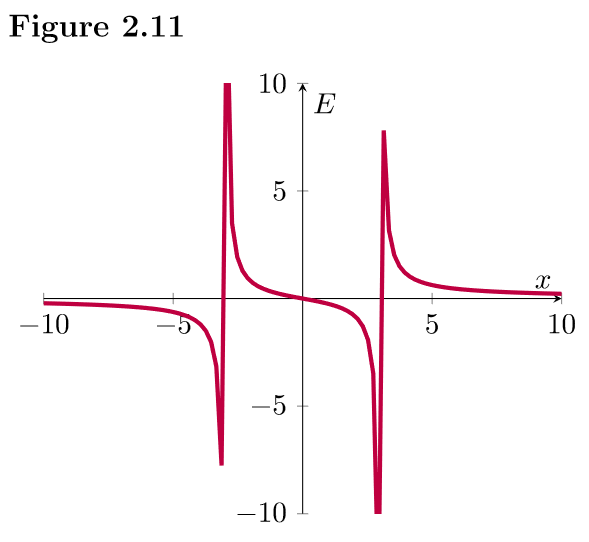
\includegraphics{Figures/Figure211}
TBA
\end{center}

\end{solution}


%%%%%%%%%%%%%%%%%%%%%%%%%%%%%%%%%%
%%%%%%%%%%%%%%%%%%%%%%%%%%%%%%%%%%
%%%%%%%%%%%%%%%%%%%%%%%%%%%%%%%%%%

\subsection*{Calculus}

\begin{question}
A charge of -Q is located at the origin, and two charges of +Q are located along the y-axis at (0,-a) and (0,a).

\begin{enumerate}[label=(\alph*)]
    \item Calculate the electric field along the x-axis, E(x)
    \item Calculate the approximate form of E(x) for very small x.
    \item Calculate the approximate form of E(x) for very large x.
\end{enumerate}
\end{question}

\begin{solution}

(A) Along the +x axis, symmetry dicates that the field must point in the x-direction. Summing the contributions of the x-components of the electric fields due to the three point charges yields the following (The vector geometry is the same as one of the previous questions. If you haven't done them, do them now!)

\begin{equation*}
    E_{net} = E_{-Q} + 2E_{+Q} \rightarrow
    E_{net} = \frac{-Q}{4\pi\epsilon_0x^2}
              +2[\frac{Q}{4\pi\epsilon_0(x^2+a^2)}
                 \frac{x}{\sqrt{x^2+a^2}}]
\end{equation*}
\begin{equation*}
    E_{net} = \frac{-Q}{4\pi\epsilon_0x^2} +
              \frac{Qx}{4\pi\epsilon_0(x^2+a^2)^{3/2}}
\end{equation*}

(B) To approximate for very small x, we will make the following approximation:

\begin{equation*}
    x^2+a^2\approx a^2
\end{equation*}

Therefore:

\begin{equation*}
    E_{net} = \frac{-Q}{4\pi\epsilon_0x^2} +
              \frac{Qx}{4\pi\epsilon_0(x^2+a^2)^{3/2}}
            \approx
            \frac{-Q}{4\pi\epsilon_0x^2} +
              \frac{Qx}{4\pi\epsilon_0 a^3}
\end{equation*}

But since:

\begin{equation*}
    \frac{1}{x^2} \gg x
\end{equation*}

Then:

\begin{equation*}
    E_{net} \approx 
                \frac{-Q}{4\pi\epsilon_0x^2} +
                \frac{Qx}{4\pi\epsilon_0 a^3}
            \approx
                \frac{-Q}{4\pi\epsilon_0x^2}
\end{equation*}

(C) To approximate for very large x, we can make a similar approximation:

\begin{equation*}
    x^2+a^2 \approx x^2
\end{equation*}

Therefore:

\begin{equation*}
    E_{net} = \frac{-Q}{4\pi\epsilon_0x^2} +
              \frac{Qx}{4\pi\epsilon_0(x^2+a^2)^{3/2}}
            \approx
              \frac{-Q}{4\pi\epsilon_0x^2} +
              \frac{Qx}{4\pi\epsilon_0x^3}
            =
              \frac{Q}{4\pi\epsilon_0x^2}
\end{equation*}

If you're not illiterate, you would have realized this is just the standard electric field equation! This is because when you are \emph{very} far away from the origin, it's impossible to see the separation of the three charges, it seems that they're all at the origin. The resulting field is due to the sum of the three charges: $Q_{effective}=Q+Q-Q=Q$, at the origin

\end{solution}

%%%%%%%%%%%%%%%%%%

\begin{question}
Consider the potential-vs-position function shown in the figure below. At which of the following points does a charge feel the greatest force in the +x direction?

\begin{center}
% \begin{tikzpicture}[scale=0.95]
% \begin{axis}[
%     axis lines=middle,
%     xmin=-4, xmax=4,
%     ymin=-2, ymax=1,
%     xlabel = $x$,
%     ylabel = $V$,
% ]
% %Below the red is defined
% \addplot [
%     domain=-10:10, 
%     samples=100, 
%     color=red,
%     style={ultra thick}
% ]
% {-2^(-x^2)};
% \addlegendentry{$V(x)$}

% \end{axis}
% \end{tikzpicture}
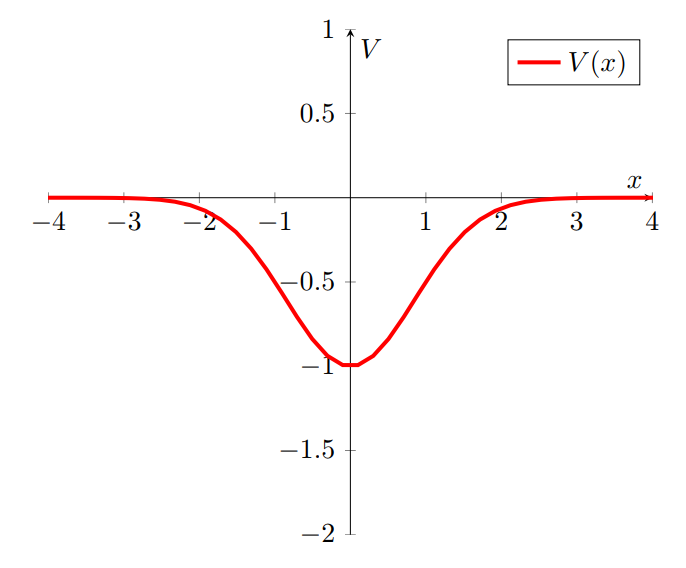
\includegraphics[scale=0.8]{Figures/Figure23}
\end{center}
\begin{multicols}{5}
\begin{enumerate}[label=(\alph*)]
    \item x=-4
    \item x=-1
    \item x=0
    \item x=1
    \item x=4
\end{enumerate}
\end{multicols}
\end{question}

\begin{solution}

Recall that the electric field is the negative slope of the potential curve: $E_x=-\frac{dV}{dx}$ so the place where the force when the slope of the potential curve has a negative value with the greatest magnitude, which is at x=-1.
\end{solution}

%%%%%%%%%%%%%%%%%%%%%%%%%%%%%%%%%%%%%%%%%%%%%%%%%%%%%%%%%%%%%%%%

\SetupExSheets{
  solution/pre-body-hook = {%
    \hyperref[qu:\CurrentQuestionID]{ (View Question)}
  }
}

%%%%%%%%%%%%%%%%%%%%%%%%%%%%%%%%%%%%%%%%%%%%%%%%%%%%%%%%%%%%%%%%

\newpage
\subsection*{Exercises}
Only answers and hints will be provided to these exercises, with no full solution. Good luck!

%%%%%%%%%%%%%%%%%%%%%%%%%%%%%%%%%%
%%%%%%%%%%%%%%%%%%%%%%%%%%%%%%%%%%
%%%%%%%%%%%%%%%%%%%%%%%%%%%%%%%%%%

\begin{question}
(AP) A conducting sphere with a radius of 0.10 meter has $1.0 \times 10^{-9}$ coulomb of charge deposited on it. the electric field just outside the surface of the sphere is:
\begin{multicols}{5}
\begin{enumerate}[label=(\alph*)]
    \item zero
    \item $450 \frac{V}{m}$
    \item $900 \frac{V}{m}$
    \item $900 \frac{V}{m}$
    \item $4500 \frac{V}{m}$
\end{enumerate}
\end{multicols}

\end{question}

\begin{solution}
C (Hint: Just like gravitation, pretend all the charge acts from the center)
\end{solution}

%%%%%%%%%%%%%%%%%%%%%%%%%%%%%%%%%%
%%%%%%%%%%%%%%%%%%%%%%%%%%%%%%%%%%
%%%%%%%%%%%%%%%%%%%%%%%%%%%%%%%%%%

\begin{question}
(AP) A positive charge +Q located at the origin produces an electric field E at point P located at (1,0). A negative charge -2Q is placed at such a point as to produce a net field of zero at point P. The second charge will be placed on the:
\begin{enumerate}[label=(\alph*)]
    \item x-axis where x > 1
    \item x-axis where 0 < x < 1
    \item x-axis where x < 0
    \item y-axis where y > 0
    \item y-axis where y < 0
\end{enumerate}

\end{question}

\begin{solution}
C (Hint: The charges have opposite signs!)
\end{solution}

%%%%%%%%%%%%%%%%%%%%%%%%%%%%%%%%%%
%%%%%%%%%%%%%%%%%%%%%%%%%%%%%%%%%%
%%%%%%%%%%%%%%%%%%%%%%%%%%%%%%%%%%

\begin{question}
(AP) Two positive charges of magnitude q are each a distance d from the origin A of a coordinate system. At which of the following points is the electric field least in magnitude?
\begin{multicols}{5}
\begin{enumerate}[label=(\alph*)]
    \item x = -d
    \item x = 0
    \item C = d
    \item D = 2d
    \item E = 3d
\end{enumerate}
\end{multicols}

\end{question}

\begin{solution}
A (Hint: Pretend it's two magnets)
\end{solution}

%%%%%%%%%%%%%%%%%%%%%%%%%%%%%%%%%%
%%%%%%%%%%%%%%%%%%%%%%%%%%%%%%%%%%
%%%%%%%%%%%%%%%%%%%%%%%%%%%%%%%%%%

\begin{question}
(AP) Two identical conducting spheres are charged to +2Q and -Q respectively, and are separated by a distance d (much greater than the radii of the spheres). The magnitude of the force of attraction of the left sphere is $F_1$. After the two spheres are made to touch and then are re-separated by distance d the magnitude of the force on the left sphere is $F_2$. Which of the following relations are true?
\begin{multicols}{5}
\begin{enumerate}[label=(\alph*)]
    \item $2F_1=F_2$
    \item $F_1=F_2$
    \item $F_1=2F_2$
    \item $F_1=4F_2$
    \item $F_1=8F_2$
\end{enumerate}
\end{multicols}

\end{question}

\begin{solution}
E (Hint: What are their charges after they touch each other?)
\end{solution}

%%%%%%%%%%%%%%%%%%%%%%%%%%%%%%%%%%
%%%%%%%%%%%%%%%%%%%%%%%%%%%%%%%%%%
%%%%%%%%%%%%%%%%%%%%%%%%%%%%%%%%%%

\begin{question}
(AP) A rigid insulated rod, with a charge of -2Q at the top and a charge of +Q at the bottom, is placed in a uniform electric field E. The rod experiences a
\begin{enumerate}[label=(\alph*)]
    \item net force to the left and a clockwise rotation
    \item net force to the left and a counterclockwise rotation
    \item net force to the right and a clockwise rotation
    \item net force to the right and a counterclockwise rotation
    \item rotation, but no net force
\end{enumerate}
\end{question}

\begin{solution}
B (Hint: in an electric field, the positive moves to the negative...)
\end{solution}

%%%%%%%%%%%%%%%%%%%%%%%%%%%%%%%%%%
%%%%%%%%%%%%%%%%%%%%%%%%%%%%%%%%%%
%%%%%%%%%%%%%%%%%%%%%%%%%%%%%%%%%%

\begin{question}
(AP) Two small spheres have equal charges q and are separated by a distance d. The force exerted on each sphere by the other has magnitude F. If the charge on each sphere is doubled and d is halved, the force on each sphere has magnitude
\begin{multicols}{5}
\begin{enumerate}[label=(\alph*)]
    \item F
    \item 2F
    \item 4F
    \item 8F
    \item 16F
\end{enumerate}
\end{multicols}

\end{question}

\begin{solution}
E (Hint: Force is proportional to $\frac{q^2}{d^2}$)
\end{solution}

%%%%%%%%%%%%%%%%%%%%%%%%%%%%%%%%%%
%%%%%%%%%%%%%%%%%%%%%%%%%%%%%%%%%%
%%%%%%%%%%%%%%%%%%%%%%%%%%%%%%%%%%

\begin{question}
(AP) A charged particle traveling with a velocity $v$ in an electric field $E$ experiences a force $F$ that must be
\begin{enumerate}[label=(\alph*)]
    \item parallel to $v$
    \item perpendicular to $v$
    \item parallel to $v \times E$
    \item parallel to $E$
    \item perpendicular to $E$
\end{enumerate}

\end{question}

\begin{solution}
E (Hint: Check out the tricks section!)
\end{solution}

%%%%%%%%

\begin{question}
(AP) A conducting sphere of radius R carries a charge Q.  Another conducting sphere has a radius R/2, but carries the same charge.  The spheres are far apart.  The ratio of the electric field near the surface of the smaller sphere to the field near the surface of the larger sphere is most nearly

\begin{multicols}{5}
\begin{enumerate}[label=(\alph*)]
    \item 1/4
    \item 1/2
    \item 1
    \item 2
    \item 4
\end{enumerate}
\end{multicols}

\end{question}

\begin{solution}
E (Hint: Use Coulomb's Law!)
\end{solution}

%%%%%%%%%%%%%%%%%%%%%%%%%%%%%%%%%%
%%%%%%%%%%%%%%%%%%%%%%%%%%%%%%%%%%
%%%%%%%%%%%%%%%%%%%%%%%%%%%%%%%%%%
\newpage
Relate to the following configurations of electric charges located at the vertices of an equilateral triangle. Use this for the next three questions:

% \begin{tikzpicture}
% \draw (0,0) -- (2,0) -- (1,1.732) -- (0,0);
% \node[below left] at (0,0) {$+q$};
% \node[below right] at (2,0) {$+q$};
% \node[above] at (1,1.732) {$+q$};
% \node[below] at (1,1) {A};

% \draw (4,0) -- (6,0) -- (5,1.732) -- (4,0);
% \node[below left] at (4,0) {$+q$};
% \node[below right] at (6,0) {$+q$};
% \node[above] at (5,1.732) {$-q$};
% \node[below] at (5,1) {B};

% \draw (8,0) -- (10,0) -- (9,1.732) -- (8,0);
% \node[below left] at (8,0) {$-q$};
% \node[below right] at (10,0) {$-q$};
% \node[above] at (9,1.732) {$+q$};
% \node[below] at (9,1) {C};

% \end{tikzpicture}

% \begin{tikzpicture}
% \draw (0,0) -- (2,0) -- (1,1.732) -- (0,0);
% \node[below left] at (0,0) {$+q$};
% \node[below right] at (2,0) {$-q$};
% \node[above] at (1,1.732) {$-2q$};
% \node[below] at (1,1) {D};

% \draw (4,0) -- (6,0) -- (5,1.732) -- (4,0);
% \node[below left] at (4,0) {$+3q$};
% \node[below right] at (6,0) {$-2q$};
% \node[above] at (5,1.732) {$-q$};
% \node[below] at (5,1) {E};

% \end{tikzpicture}
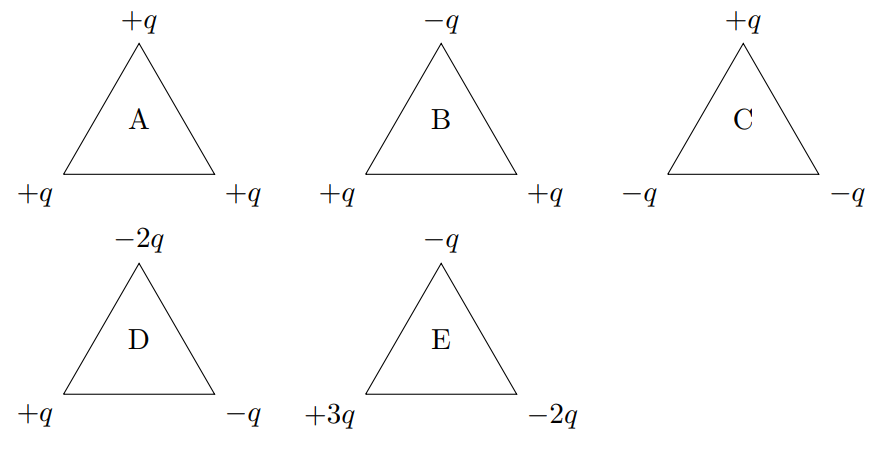
\includegraphics{Figures/Figure24}

%%%%%%%%%%%%%%%%%%%%%%%%%%%%%%%%%%
%%%%%%%%%%%%%%%%%%%%%%%%%%%%%%%%%%
%%%%%%%%%%%%%%%%%%%%%%%%%%%%%%%%%%

\begin{question}
(AP) The electric field at the center is zero at..

\begin{multicols}{5}
\begin{enumerate}[label=(\alph*)]
    \item A
    \item B
    \item C
    \item D
    \item E
\end{enumerate}
\end{multicols}

\end{question}

\begin{solution}
A (Hint: Don't overthink it! Use common sense if you have any)
\end{solution}

%%%%%%%%%%%%%%%%%%%%%%%%%%%%%%%%%%
%%%%%%%%%%%%%%%%%%%%%%%%%%%%%%%%%%
%%%%%%%%%%%%%%%%%%%%%%%%%%%%%%%%%%

\begin{question}
(AP) The electric field at the center is zero at..

\begin{multicols}{5}
\begin{enumerate}[label=(\alph*)]
    \item A
    \item B
    \item C
    \item D
    \item E
\end{enumerate}
\end{multicols}

\end{question}

\begin{solution}
C (Hint: Make use of superposition, and remember which way the electric field points!)
\end{solution}

%%%%%%%%%%%%%%%%%%%%%%%%%%%%%%%%%%
%%%%%%%%%%%%%%%%%%%%%%%%%%%%%%%%%%
%%%%%%%%%%%%%%%%%%%%%%%%%%%%%%%%%%

\begin{question}
The electric potential at the center is zero at...
\begin{multicols}{5}
\begin{enumerate}[label=(\alph*)]
    \item A
    \item B
    \item C
    \item D
    \item E
\end{enumerate}
\end{multicols}

\end{question}

\begin{solution}
E (Hint: Potential is a scaler!)
\end{solution}

%%%%%%%%%%%%%%%%%%%%%%%%%%%%%%%%%%
%%%%%%%%%%%%%%%%%%%%%%%%%%%%%%%%%%
%%%%%%%%%%%%%%%%%%%%%%%%%%%%%%%%%%

\begin{question}
(AP) From the electric field vector at a point, one can determine which of the following at that point?

\begin{enumerate}
    \item The direction of the electrostatic force on a test charge of known sign
    \item The magnitude of the electrostatic force exerted per unit charge on a test charge
    \item The electrostatic charge
\end{enumerate}

\begin{multicols}{5}
\begin{enumerate}[label=(\alph*)]
    \item I
    \item III 
    \item I \& II
    \item II \& III
    \item All 3
\end{enumerate}
\end{multicols}

\end{question}

\begin{solution}
C (Hint: Review what an electric field is!)
\end{solution}

%%%%%%%%%%%%%%%%%%%%%%%%%%%%%%%%%%
%%%%%%%%%%%%%%%%%%%%%%%%%%%%%%%%%%
%%%%%%%%%%%%%%%%%%%%%%%%%%%%%%%%%%

\begin{question}
(AP) A circular ring made of an insulating material is cut in half.  One half is given a charge -q uniformly distributed along its arc.  The other half is given a charge +q also uniformly distributed along its arc.  The two halves are then rejoined with insulation at the junctions J, as shown above.  If there is no change in the charge distributions, what is the direction of the net electrostatic force on an electron located at the center of the circle? 
\begin{enumerate}[label=(\alph*)]
    \item Toward the top of the page
    \item Toward the bottom of the page
    \item To the right
    \item To the left
    \item Into the page
\end{enumerate}

\end{question}

\begin{solution}
B (Hint: Draw it out!)
\end{solution}

%%%%%%%%%%%%%%%%%%%%%%%%%%%%%%%%%%
%%%%%%%%%%%%%%%%%%%%%%%%%%%%%%%%%%
%%%%%%%%%%%%%%%%%%%%%%%%%%%%%%%%%%

\begin{question}
(AP) Two metal spheres are initially uncharged are mounted on insulating stands. A negatively charged rubber rod is brought close to, but does not make contact with, sphere X. Sphere Y is then brought close to X on the side opposite to the rod. Y is allowed to touch X and then is removed far away. The rubber rod is then moved far away from X and Y. What are the final charges on the spheres?

\begin{center}
\begin{tabular}{ |c|c|c| } 
 \hline
       & Sphere X & Sphere Y \\ 
 A      & Zero  & Zero  \\ 
 B      & Negative  & Negative  \\ 
 C      & Negative  & Positive  \\ 
 D      & Positive  & Negative  \\ 
 E      & Positive  & Positive  \\ 

 \hline
\end{tabular}
\end{center}

\end{question}

\begin{solution}
D (Hint: Draw it out. Protons can't move!)
\end{solution}

%%%%%%%%%%%%%%%%%%%%%%%%%%%%%%%%%%
%%%%%%%%%%%%%%%%%%%%%%%%%%%%%%%%%%
%%%%%%%%%%%%%%%%%%%%%%%%%%%%%%%%%%

\begin{question}
(AP) Two initially uncharged conductors, 1 and 2, are mounted on insulating stands and are in contact. A negatively charged rod is brought near conductor 1, at the opposite side of conductor 2, but does not touch them. With the rod held in place, conductor 2 is moved to the right by pushing its stand, so the conductors are separated. Which of the following is now true about the charge of conductor 2?
\begin{multicols}{5}
\begin{enumerate}[label=(\alph*)]
    \item no charge
    \item positive
    \item negative
    \item unknown
    \item no change
\end{enumerate}
\end{multicols}

\end{question}

\begin{solution}
E (Hint: Potential is a scaler!)
\end{solution}

%%%%%%%%%%%%%%%%%%%%%%%%%%%%%%%%%%
%%%%%%%%%%%%%%%%%%%%%%%%%%%%%%%%%%
%%%%%%%%%%%%%%%%%%%%%%%%%%%%%%%%%%
\newpage
As shown below, two particles, each of charge +Q, are fixed at opposite corners of a square that lies in the plane of the page. A positive test charge +q is placed at a third corner. Use this information for the next two questions.

\begin{center}
% \begin{tikzpicture}
% \draw (0,0) -- (0,2) -- (2,2) -- (2,0) -- (0,0);
% \node[above right] at (0,0) {$+q$};
% \node[below right] at (0,2) {$+Q$};
% \node[above left] at (2,0) {$+Q$};
% \end{tikzpicture}
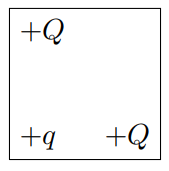
\includegraphics{Figures/Figure25}
\end{center}

%%%%%%%%%%%%%%%%%%%%%%%%%%%%%%%%%%
%%%%%%%%%%%%%%%%%%%%%%%%%%%%%%%%%%
%%%%%%%%%%%%%%%%%%%%%%%%%%%%%%%%%%

\begin{question}
(AP) What is the direction of the force on the test charge due to the two other charges?

\begin{enumerate}[label=(\alph*)]
    \item top right
    \item right
    \item bottom right
    \item down
    \item bottom left
\end{enumerate}

\end{question}

\begin{solution}
E (Hint: Look at the force exerted by each individual particle first)
\end{solution}

%%%%%%%%%%%%%%%%%%%%%%%%%%%%%%%%%%
%%%%%%%%%%%%%%%%%%%%%%%%%%%%%%%%%%
%%%%%%%%%%%%%%%%%%%%%%%%%%%%%%%%%%

\begin{question}
(AP) If F is the magnitude of the force on the test charge due to only one of the other charges, what is the magnitude of the net force acting on the test charge due to both of these charges?
\begin{multicols}{5}
\begin{enumerate}[label=(\alph*)]
    \item Zero
    \item $\frac{F}{\sqrt{2}}$
    \item F
    \item $\sqrt{2}$F
    \item 2
\end{enumerate}
\end{multicols}

\end{question}

\begin{solution}
D (Hint: Why isn't it 2F? First calculate vector form, then convert to magnitude)
\end{solution}


%%%%%%%%%%%%%%%%%%%%%%%%%%%%%%%%%%
%%%%%%%%%%%%%%%%%%%%%%%%%%%%%%%%%%
%%%%%%%%%%%%%%%%%%%%%%%%%%%%%%%%%%

\begin{question}
(AP) If the only force acting on an electron is due to a uniform electric field, the electron moves with constant
\begin{enumerate}[label=(\alph*)]
    \item acceleration in a direction opposite to that of the field
    \item acceleration in the direction of the field
    \item acceleration in a direction perpendicular to that of the field
    \item speed in a direction opposite to that of the field
    \item speed in the direction of the field
\end{enumerate}

\end{question}

\begin{solution}
A (Hint: Which ways to field lines point again?)
\end{solution}

%%%%%%%%%%%%%%%%%%%%%%%%%%%%%%%%%%
%%%%%%%%%%%%%%%%%%%%%%%%%%%%%%%%%%
%%%%%%%%%%%%%%%%%%%%%%%%%%%%%%%%%%
\newpage
Particle of charge Q is located at (-2,0) and another particle of charge -4Q is located at (2,0). Assume the particles are isolated from all other charges. P is a point on the y axis above the x axis. Use this information to answer the next two questions:

%%%%%%%%%%%%%%%%%%%%%%%%%%%%%%%%%%
%%%%%%%%%%%%%%%%%%%%%%%%%%%%%%%%%%
%%%%%%%%%%%%%%%%%%%%%%%%%%%%%%%%%%
\begin{question}
(AP) Which of the following describes the direction of the electric field at point P
\begin{multicols}{5}
\begin{enumerate}[label=(\alph*)]
    \item +x
    \item +y
    \item -y
    \item -x and +y
    \item +x and -y
\end{enumerate}
\end{multicols}

\end{question}

\begin{solution}
E (Hint: Draw your electric field lines! Remember the charges aren't equal.)
\end{solution}

%%%%%%%%%%%%%%%%%%%%%%%%%%%%%%%%%%
%%%%%%%%%%%%%%%%%%%%%%%%%%%%%%%%%%
%%%%%%%%%%%%%%%%%%%%%%%%%%%%%%%%%%

\begin{question}
(AP) At which of the following points on the x-axis is the electric field zero?
\begin{multicols}{5}
\begin{enumerate}[label=(\alph*)]
    \item (-6,0)
    \item (-3,0)
    \item (-1,0)
    \item (1,0)
    \item (6,0)
\end{enumerate}
\end{multicols}

\end{question}

\begin{solution}
A (Hint: Draw MOARRR lines! Or superimpose the electric field equation. Your choice.)
\end{solution}

%%%%%%%%%%%%%%%%%%%%%%%%%%%%%%%%%%
%%%%%%%%%%%%%%%%%%%%%%%%%%%%%%%%%%
%%%%%%%%%%%%%%%%%%%%%%%%%%%%%%%%%%

\begin{question}
(AP) When a negatively charged rod is brought near, but does not touch, an initially uncharged electroscope, the leaves spring apart. (I) When the electroscope is then touched with a finger, the leaves collapse. When the finger and finally the rod are removed, the leaves spring apart a second time (II). The charge on the leaves is:
\begin{enumerate}[label=(\alph*)]
    \item positive in both I and II
    \item negative in I and III
    \item positive in I, negative in III
    \item negative in I, positive in III
    \item impossible to determine in either I or III
\end{enumerate}

\end{question}

\begin{solution}
E (Hint: Draw it out! It's first charging by separation then charging by induction)
\end{solution}

%%%%%%%%%%%%%%%%%%%%%%%%%%%%%%%%%%
%%%%%%%%%%%%%%%%%%%%%%%%%%%%%%%%%%
%%%%%%%%%%%%%%%%%%%%%%%%%%%%%%%%%%
\newpage
\begin{question}
Two experiments are performed using a pair of solid metal spheres connected by a switch. Both spheres are grounded before each experiment so that they initially have no charge.

\emph{Experiment I:} A positively charged rod is brought near sphere A while the the switch is closed, the switch is opened, and the rod is then removed.

\emph{Experiment II:} A positively charged rod is touched to sphere A while the switch is closed, the switch is opened, and the rod is then removed.

Which of the following describes the charge on the spheres after both experiments?
\begin{enumerate}[label=(\alph*)]
    \item After I: both have no charge; After II: both are positive
    \item After I: A is negative and B is positive; After II: A is positive and B is negative
    \item After I: A is negative and B is positive; After II: both are positive
    \item After I and II: both are positive
    \item After I and II: A is positive and B is negative
\end{enumerate}

\end{question}

\begin{solution}
C (Hint: There's a lot going on. Draw lots of diagrams, and use a process of elmination!)
\end{solution}

%%%%%%%%%%%%%%%%%%%%%%%%%%%%%%%%%%
%%%%%%%%%%%%%%%%%%%%%%%%%%%%%%%%%%
%%%%%%%%%%%%%%%%%%%%%%%%%%%%%%%%%%
%%%%%%%%%%%%%%%%%%%%%%%%%%%%%%%%%%
%%%%%%%%%%%%%%%%%%%%%%%%%%%%%%%%%%
%%%%%%%%%%%%%%%%%%%%%%%%%%%%%%%%%%
%%%%%%%%%%%%%%%%%%%%%%%%%%%%%%%%%%
%%%%%%%%%%%%%%%%%%%%%%%%%%%%%%%%%%
%%%%%%%%%%%%%%%%%%%%%%%%%%%%%%%%%%
%%%%%%%%%%%%%%%%%%%%%%%%%%%%%%%%%%
%%%%%%%%%%%%%%%%%%%%%%%%%%%%%%%%%%
%%%%%%%%%%%%%%%%%%%%%%%%%%%%%%%%%%
%%%%%%%%%%%%%%%%%%%%%%%%%%%%%%%%%%
%%%%%%%%%%%%%%%%%%%%%%%%%%%%%%%%%%
%%%%%%%%%%%%%%%%%%%%%%%%%%%%%%%%%%

\newpage
\section{Solutions}


\printsolutions

\newpage
\section{Solutions}
\printsolutions

\end{document}